\documentclass{article}
\usepackage{amsmath}
\usepackage{amsfonts} 
\usepackage{physics} 
\usepackage{rotating}
\usepackage{enumitem}
\setlength{\headheight}{15pt}
\usepackage[italian]{varioref}
\usepackage{hyperref}
\usepackage{steinmetz}
\hypersetup{colorlinks=true, linkcolor=magenta, citecolor=green, urlcolor=blue} 
\usepackage{mathtools}
\hypersetup{linktoc=page}
\usepackage{extramarks}
\usepackage{amssymb}
\usepackage{fancyhdr}
\usepackage{float}
\usepackage{geometry}
 \geometry{
 a4paper,
 total={190mm,257mm},
 left=15mm,
 right=15mm,
 top=20mm,
 }
\usepackage{graphicx}
\graphicspath{ {./images/} }
\usepackage{amsthm}
\usepackage{etoolbox}
\BeforeBeginEnvironment{minipage}{\medskip}
\AfterEndEnvironment{minipage}{\medskip}
\usepackage{tocloft}
\usepackage{indentfirst}
\usepackage{tikz}
\usepackage{afterpage}
\numberwithin{equation}{section}
\newcommand\blankpage{%
    \null
    \thispagestyle{empty}%
    \addtocounter{page}{-1}%
    \newpage}
\newcommand\blankpagewnumber{%
    \null
    \newpage}
\newcommand{\R}{\mathbb{R}}
\newcommand{\T}{\mathcal{T}}
\newcommand{\U}{\mathcal{U}}
\renewcommand{\L}{\mathcal{L}}
\usepackage{blkarray, bigstrut}
\usepackage[T1]{fontenc}

\begin{document}
\afterpage{\blankpage}
\begin{titlepage}
\begin{center}
\huge Master's degree in Computer Engineering for Robotics and Smart Industry
\end{center}
\vspace*{\fill}
\begin{center}
\textbf{\Huge Physical Human-Robot Interaction}
\end{center}
\begin{center}
Report on the assignments given during the 2022/2023 a.y.
\end{center}
\vspace*{\fill}
\begin{center}
\begin{minipage}{0.4\textwidth}
\begin{flushleft}
Author: Lorenzo Busellato, VR472249\\
email: lorenzo.busellato\_02@studenti.univr.it
\end{flushleft}
\end{minipage}
\begin{minipage}{0.5\textwidth}
\begin{flushright}

\includegraphics[keepaspectratio,width=0.6\textwidth]{logo}
\end{flushright}
\end{minipage}

\end{center}
\vspace{1cm}
\end{titlepage}


\afterpage{\blankpage}
\thispagestyle{empty}
\setcounter{page}{0}
\pagenumbering{gobble}
\renewcommand{\cftsecleader}{\cftdotfill{\cftdotsep}}
\setcounter{tocdepth}{2}
\tableofcontents
\clearpage

\fancyhead[R]{}
\fancyhead[L]{}
\pagestyle{fancy}
\pagenumbering{arabic}

\section{Assignment 1}

\subsection{Implement the single-input single-output four-channel bilateral teleoperation architecture}

\begin{figure}[h]
\centering
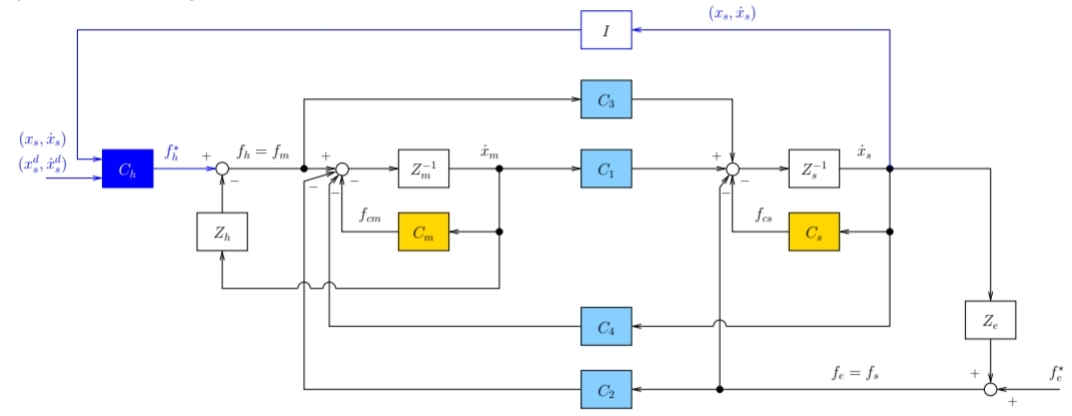
\includegraphics[keepaspectratio,width=0.9\textwidth]{4ch_arch}
\caption{SISO 4ch bilateral teleoperation architecture}
\end{figure}

The inner controllers for the robots are defined as follows:
\begin{equation*}
C_m=B_m+\frac{K_m}{s}\;\;\;\;\;\;C_s=B_s+\frac{K_s}{s}
\end{equation*}

To achieve perfect transparency, the coordination controllers must satisfy the following conditions:
\begin{align*}
\begin{cases}
C_1&=Z_s+C_s\\
C_2&=I\\
C_3&=I\\
C_4&=-(Z_m+C_m)
\end{cases}\;\;\;\;\text{with }Z_m=M_ms+D_m,\;Z_s=M_ss+D_s
\end{align*}

with $M_m=0.5,M_s=2,D_m=D_s=0$.

The human is modelled  with damping $B_h=1$ and stiffness $K_h=0$. The human intention is modelled with a PD controller with $K_P=2000$ and $K_D=50$. The master robot is controlled with a PD controller with $K_P=20$ and $K_D=10$. The slave robot is controlled with a PD controller with $K_P=4000$ and $K_D=500$.

The environment is modelled as a spring with  inertia $B_e=100$ and stiffness $K_e=200$.

The architecture is tested with a low-pass filtered step signal ($f_{lp}=0.5$Hz, $A=1$) and with a sinusoidal signal ($A=1$, $f=1$Hz), both in free motion ($x_e = 1.5$) and in contact ($x_e = 0.75$). The architecture is tested both with $D_m=D_s=0$ and $D_m=5,D_s=10$.

The architecture is modeled in simulink as follows:

\begin{figure}[H]
\centering
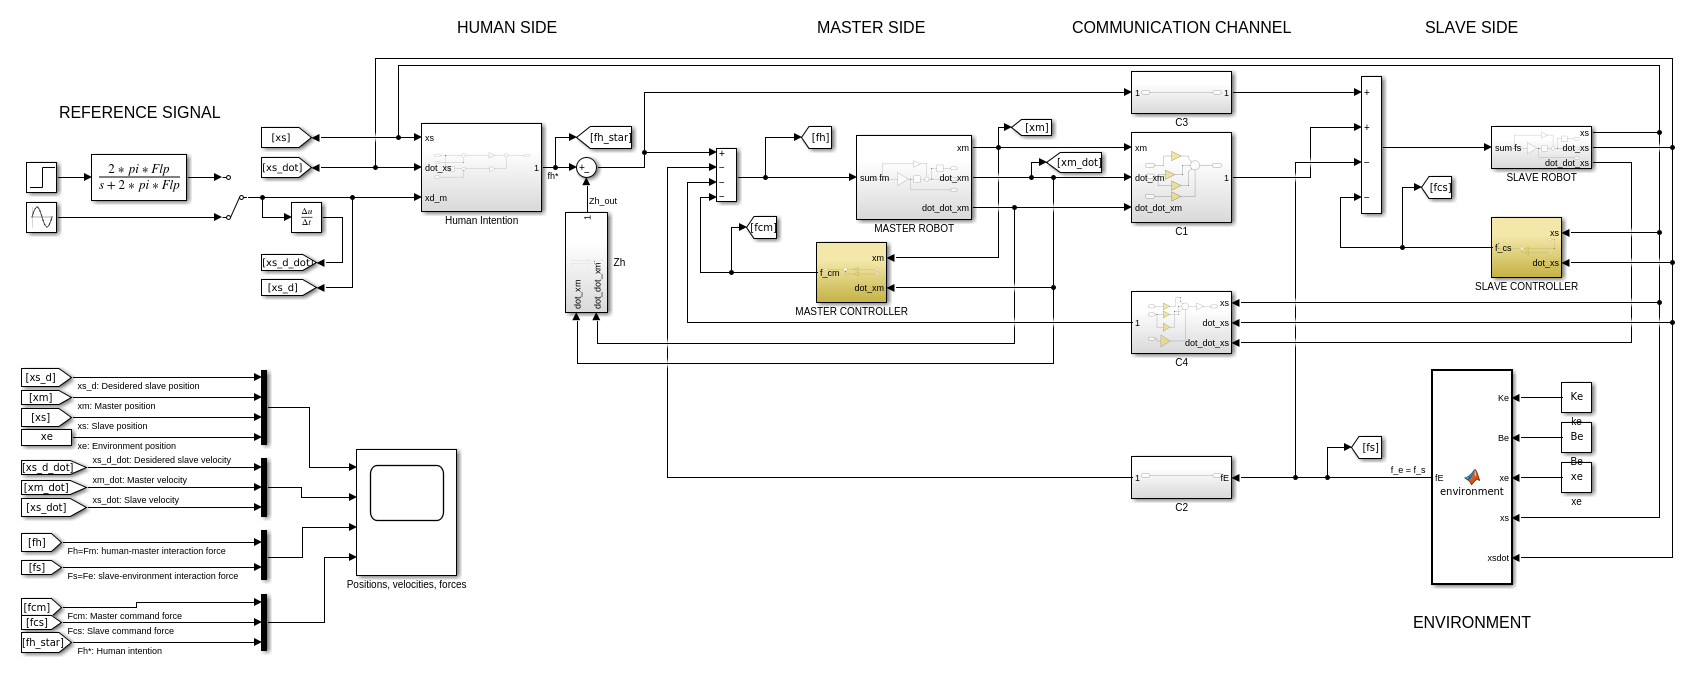
\includegraphics[keepaspectratio,width=0.85\textwidth]{4ch_simulink}
\caption{SISO 4ch bilateral teleoperation architecture - SIMULINK model}
\end{figure}

\newpage

\begin{figure}[H]
\begin{minipage}{0.5\textwidth}
\begin{figure}[H]
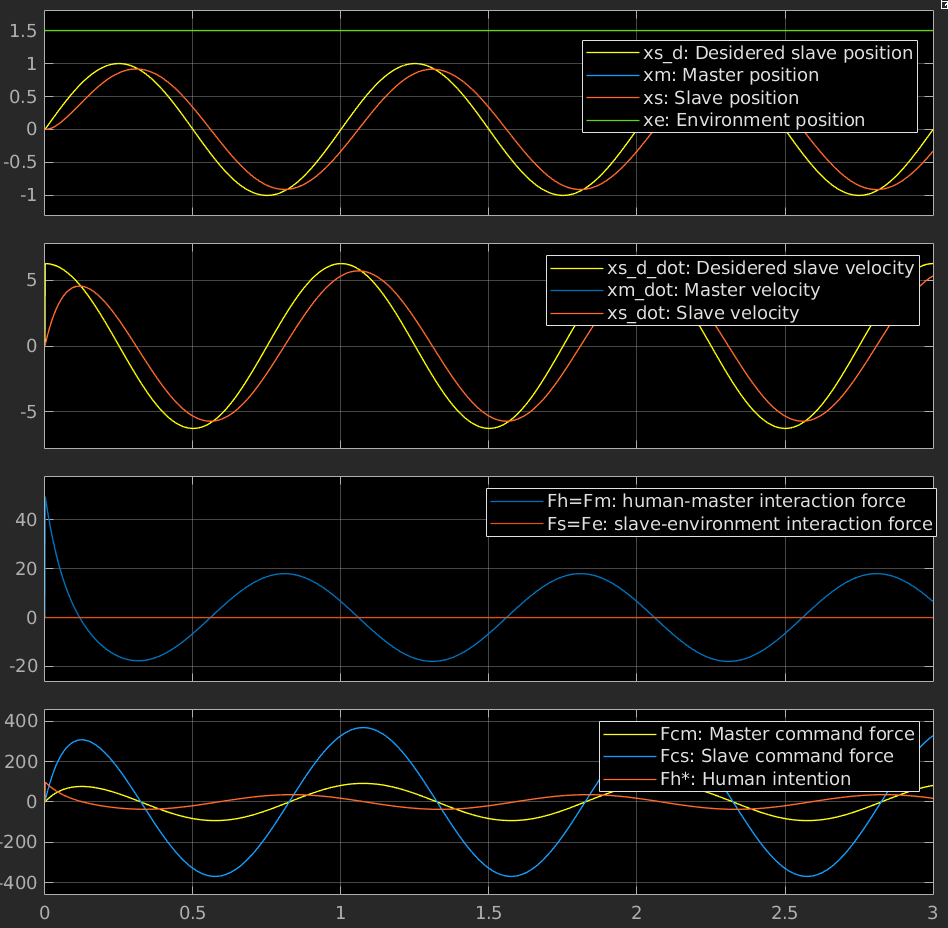
\includegraphics[keepaspectratio,width=\textwidth]{sin_free_nod}
\caption{Sinusoidal response in free motion\\ with $Dm=Ds=0$}
\label{fig:sin_free_nod}
\end{figure}
\begin{figure}[H]
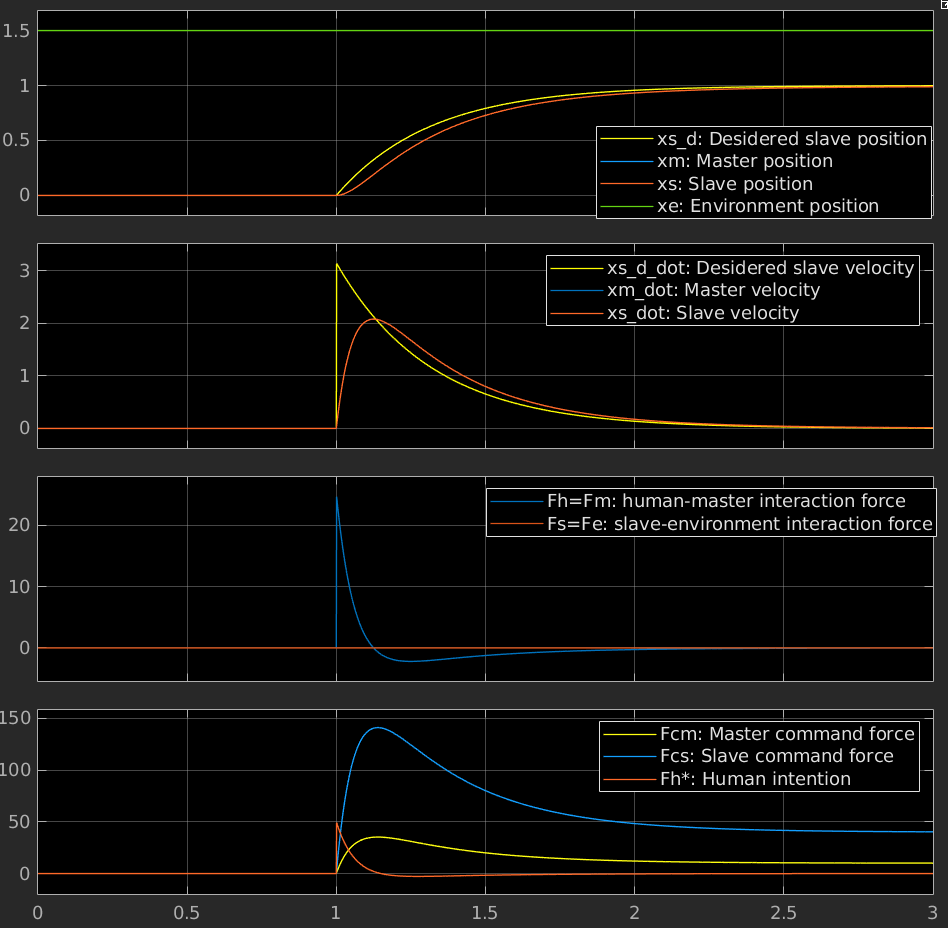
\includegraphics[keepaspectratio,width=\textwidth]{step_free_nod}
\caption{Step response in free motion with $Dm=Ds=0$}
\label{fig:step_free_nod}
\end{figure}
\end{minipage}
\begin{minipage}{0.5\textwidth}
\begin{figure}[H]
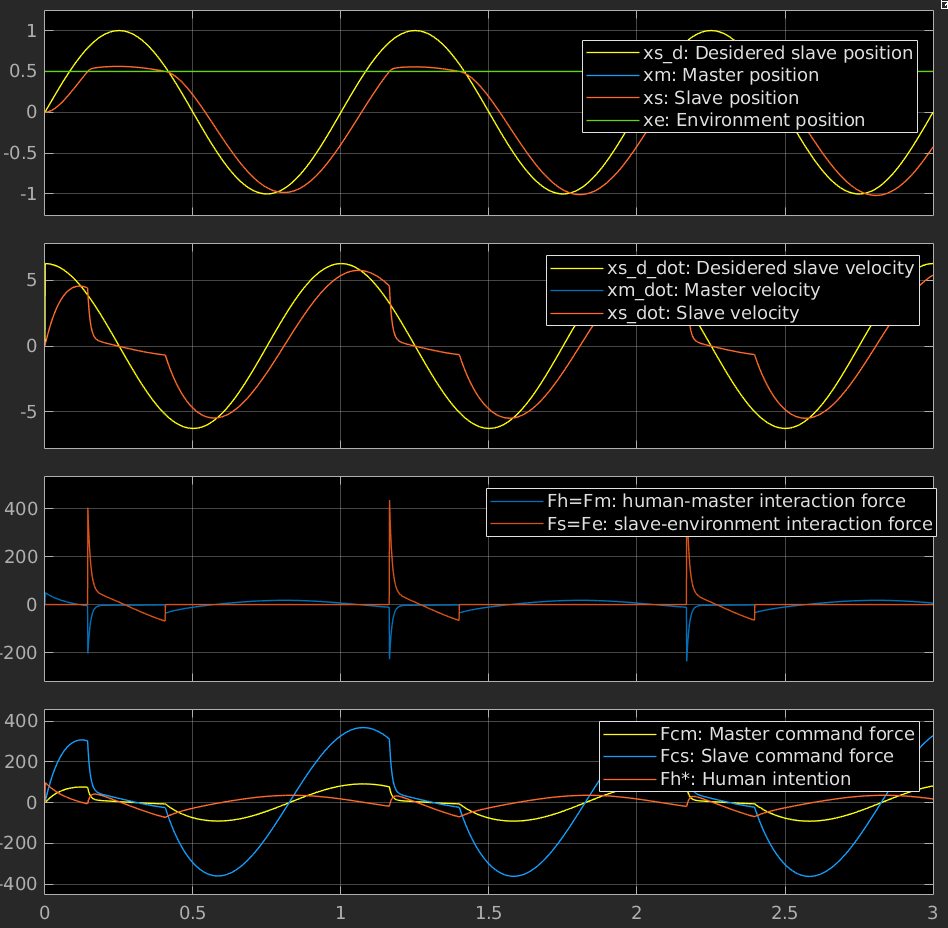
\includegraphics[keepaspectratio,width=\textwidth]{sin_contact_nod}
\caption{Sinusoidal response in contact\\ with $Dm=Ds=0$}
\label{fig:sin_contact_nod}
\end{figure}
\begin{figure}[H]
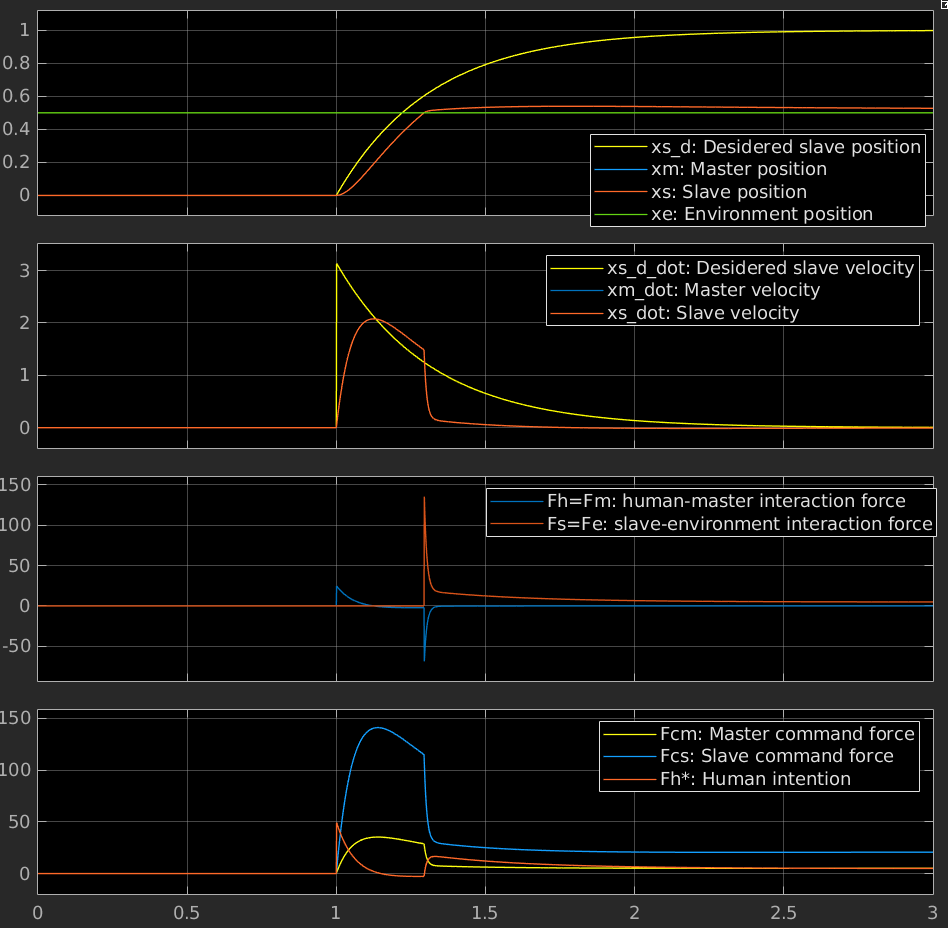
\includegraphics[keepaspectratio,width=\textwidth]{step_contact_nod}
\caption{Step response in contact with $Dm=Ds=0$}
\label{fig:step_contact_nod}
\end{figure}
\end{minipage}
\end{figure}

In both the sinusoidal and step reference cases, the trajectory is followed with some delay in free motion (figures \ref{fig:sin_free_nod} and \ref{fig:step_free_nod}). In contact (figures \ref{fig:sin_contact_nod} and \ref{fig:step_contact_nod}), once the slave reaches the environment there are sharp spikes in the force of both slave and master, and the trajectory is no longer followed during contact. In all cases, under the condition of perfect transparency, the slave and master robots positions are the same.

\newpage

\begin{figure}[H]
\begin{minipage}{0.5\textwidth}
\begin{figure}[H]
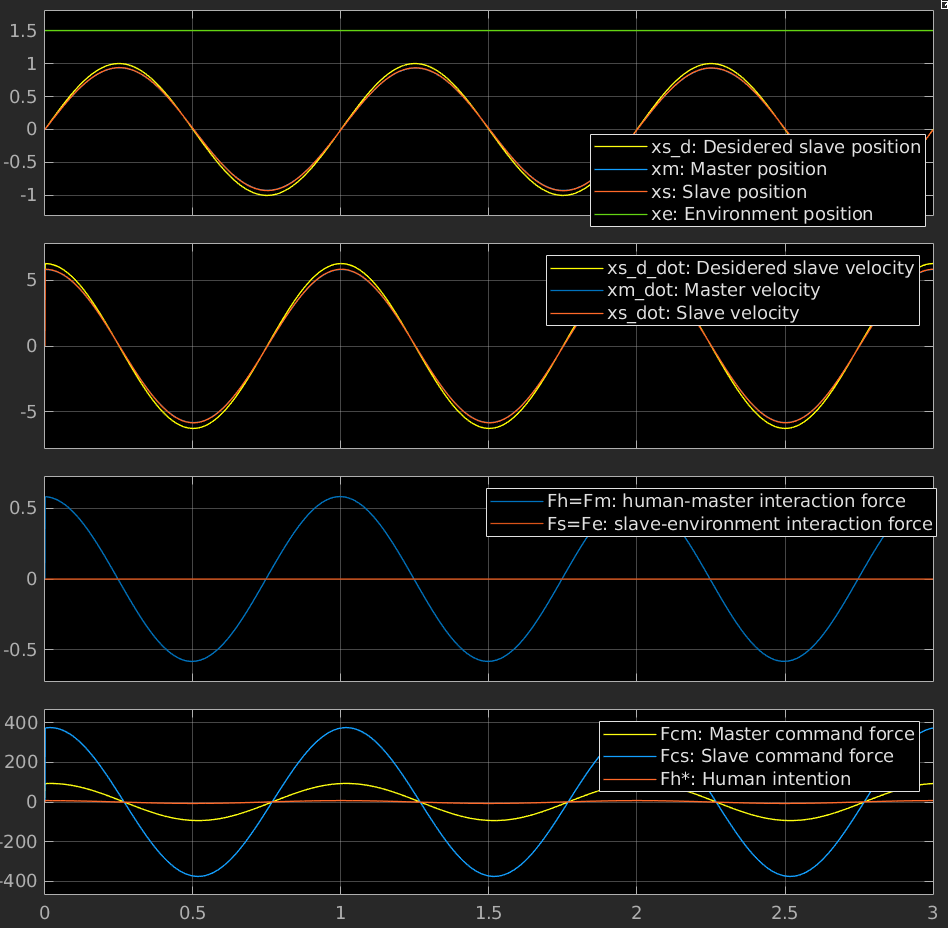
\includegraphics[keepaspectratio,width=\textwidth]{sin_free_d}
\caption{Sinusoidal response in free motion\\ with $Dm=5,Ds=10$}
\label{fig:sin_free_d}
\end{figure}
\begin{figure}[H]
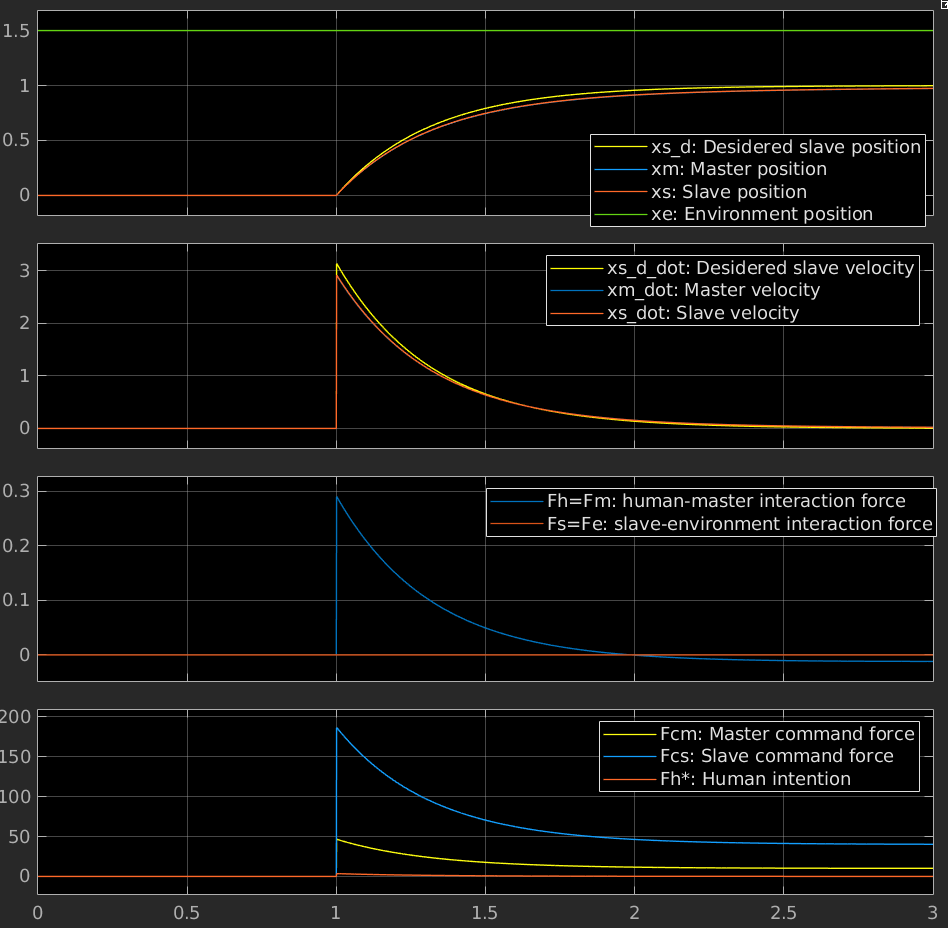
\includegraphics[keepaspectratio,width=\textwidth]{step_free_d}
\caption{Step response in free motion\\ with $Dm=5,Ds=10$}
\label{fig:step_free_d}
\end{figure}
\end{minipage}
\begin{minipage}{0.5\textwidth}
\begin{figure}[H]
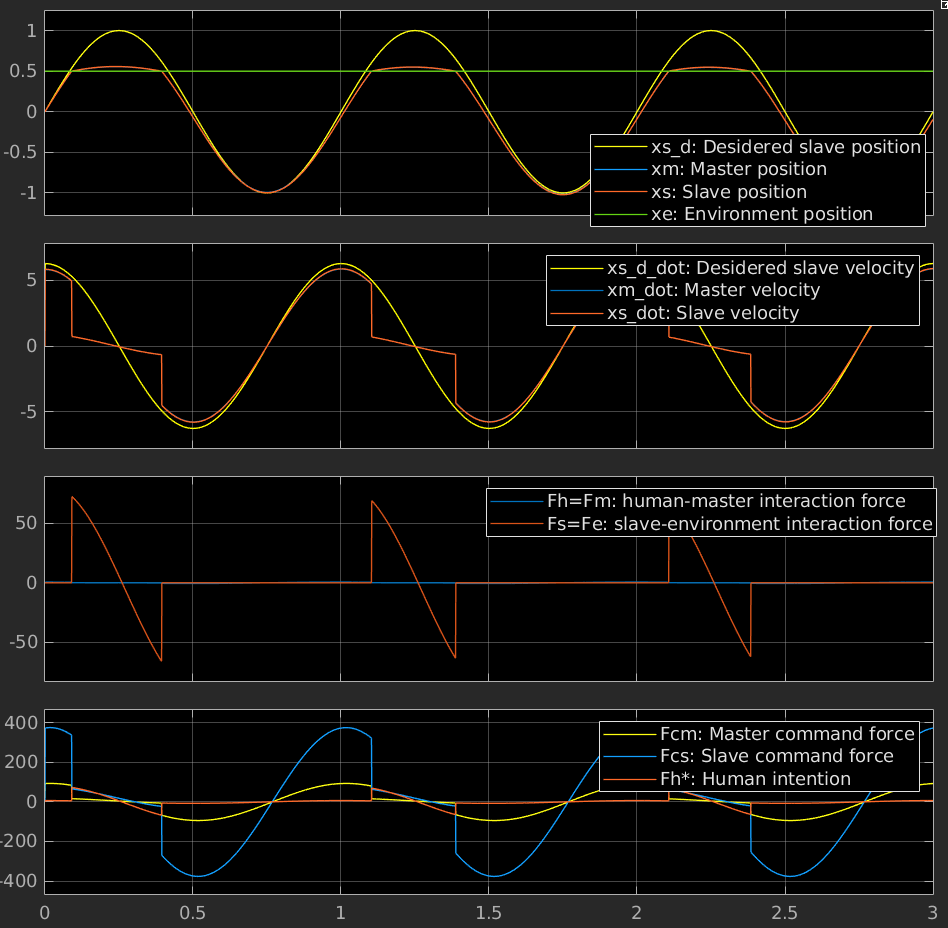
\includegraphics[keepaspectratio,width=\textwidth]{sin_contact_d}
\caption{Sinusoidal response in contact\\ with $Dm=5,Ds=10$}
\label{fig:sin_contact_d}
\end{figure}
\begin{figure}[H]
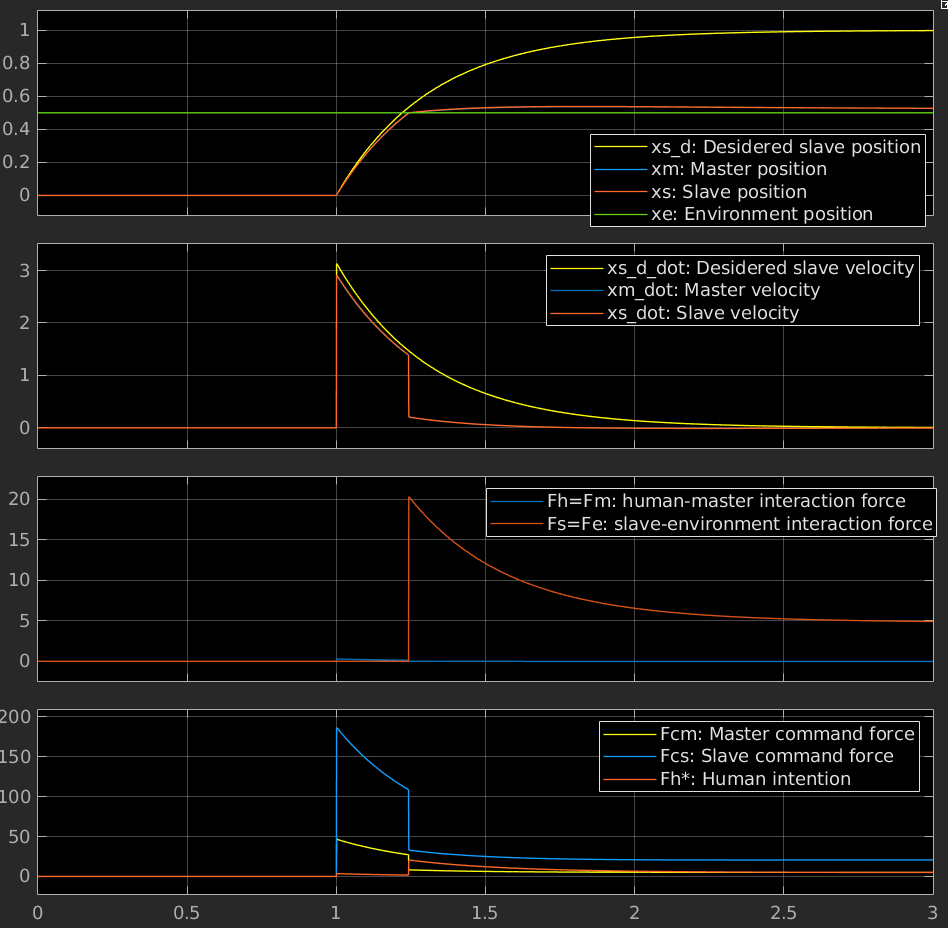
\includegraphics[keepaspectratio,width=\textwidth]{step_contact_d}
\caption{Step response in contact\\\hspace{\textwidth} with $Dm=5,Ds=10$}
\label{fig:step_contact_d}
\end{figure}
\end{minipage}
\end{figure}

Using damping values of $D_m=5,D_s=10$ improves the trajectory execution, both in the free motion (figures \ref{fig:sin_free_d} and \ref{fig:step_free_d}) and contact (figures \ref{fig:sin_contact_d} and \ref{fig:step_contact_d}) cases. Additionally the force spikes observed in the contact case are reduced.

\newpage

\section{Assignment 2}

\subsection{Implement the three two-channel bilateral teleoperation architectures and the three-channel bilateral teleoperation architecture}

The three two-channel architectures and the three channel architecture are obtained by removing some of the coordinating controllers:

\begin{itemize}
\item 2-channel position-position (P-P): $C_2=C_3=0$
\item 2-channel force-position (F-P): $C_3=C_4=0$
\item 2-channel force-force (F-F): $C_1=C_4=0$
\item 3-channel position and force-position (P,F-P): $C_3=0$
\end{itemize}

The four architectures are modelled with the same SIMULINK model, which is based on the 4-channel architecture, with the added possibility of individually cutting off the coordinating controllers:

\begin{figure}[H]
\centering
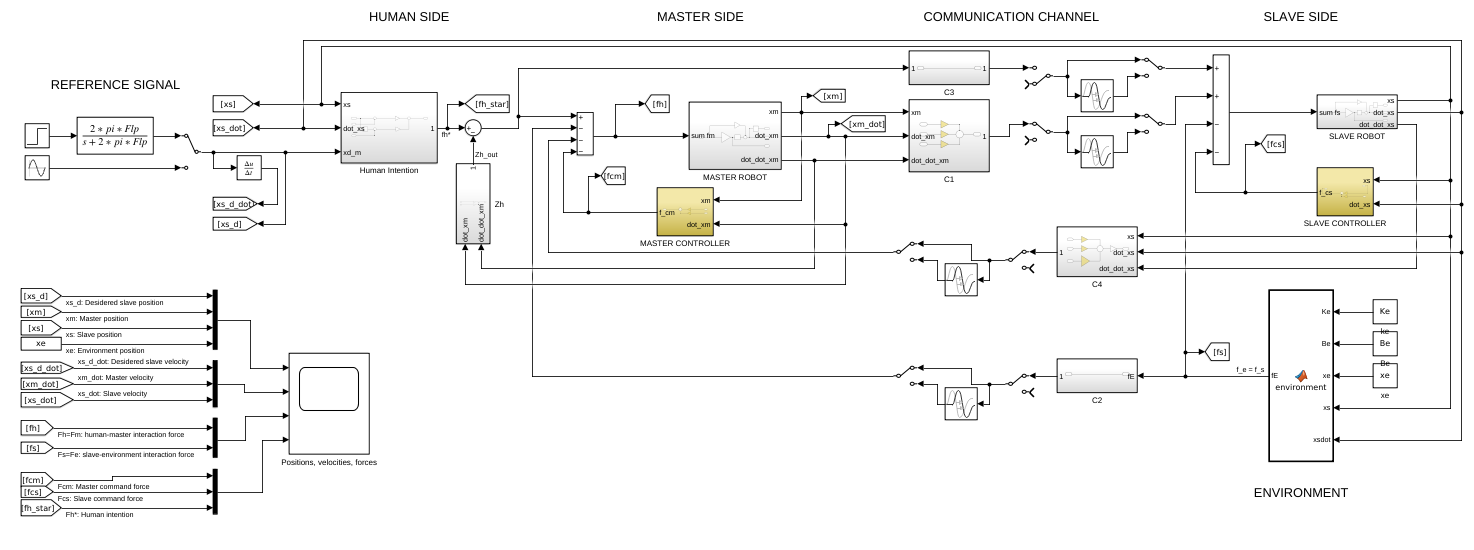
\includegraphics[keepaspectratio,width=0.9\textwidth]{2_3_ch_arch}
\caption{2-3 channel teleoperation architecture with transport delays - SIMULINK model}
\end{figure}

\newpage

\begin{figure}[H]
\begin{minipage}{0.5\textwidth}
\begin{figure}[H]
\centering
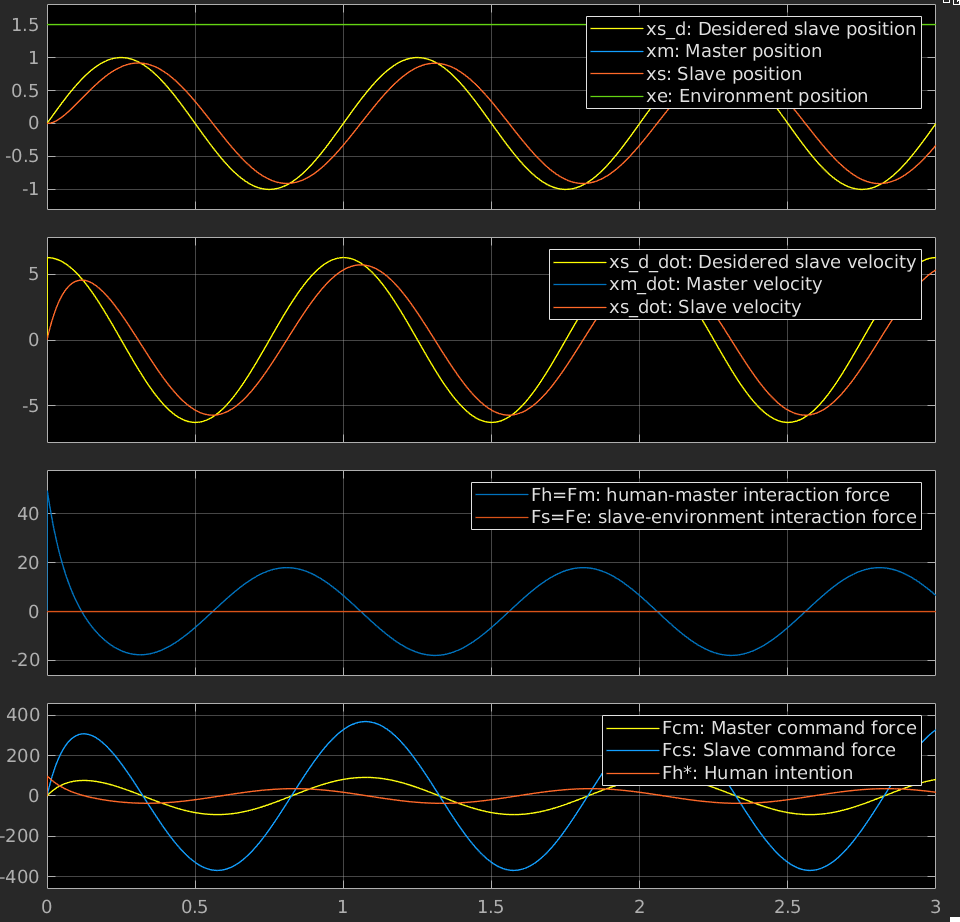
\includegraphics[keepaspectratio,width=\textwidth]{PP_free_nod}
\caption{2-channel P-P in free motion.}
\label{fig:pp_free}
\end{figure}
\begin{figure}[H]
\centering
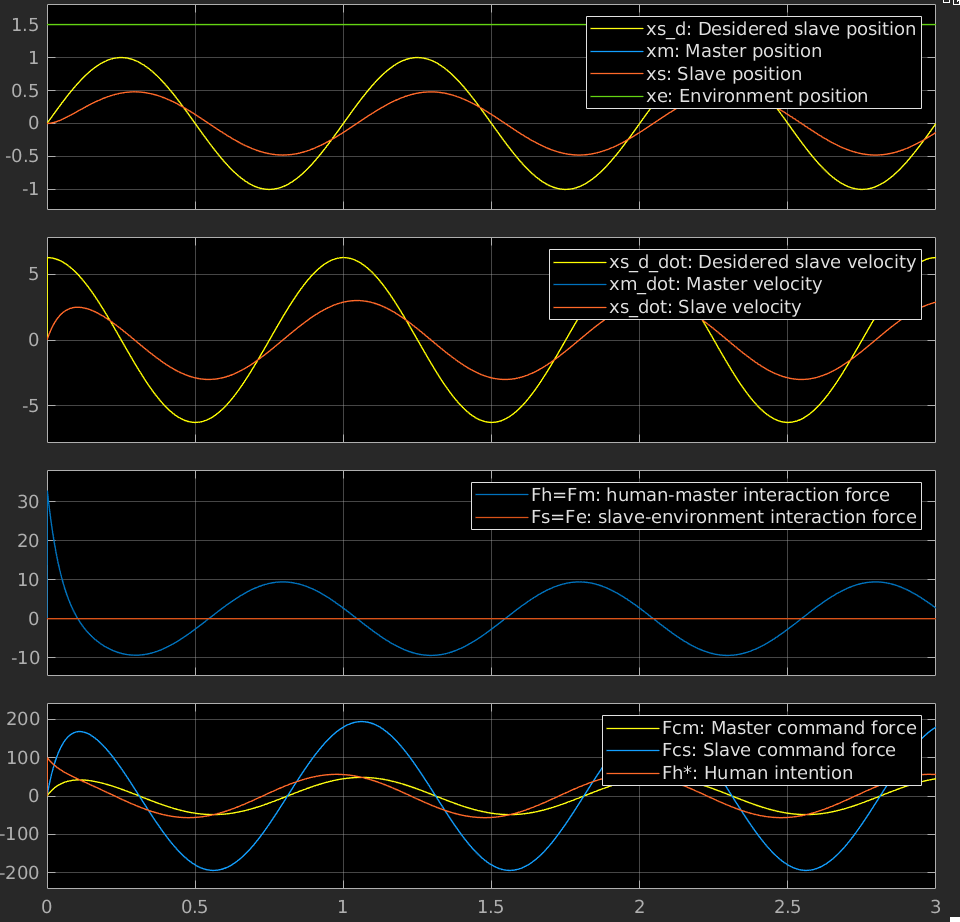
\includegraphics[keepaspectratio,width=\textwidth]{FP_free_nod}
\caption{2-channel F-P in free motion.}
\label{fig:fp_free}
\end{figure}
\end{minipage}
\begin{minipage}{0.5\textwidth}
\begin{figure}[H]
\centering
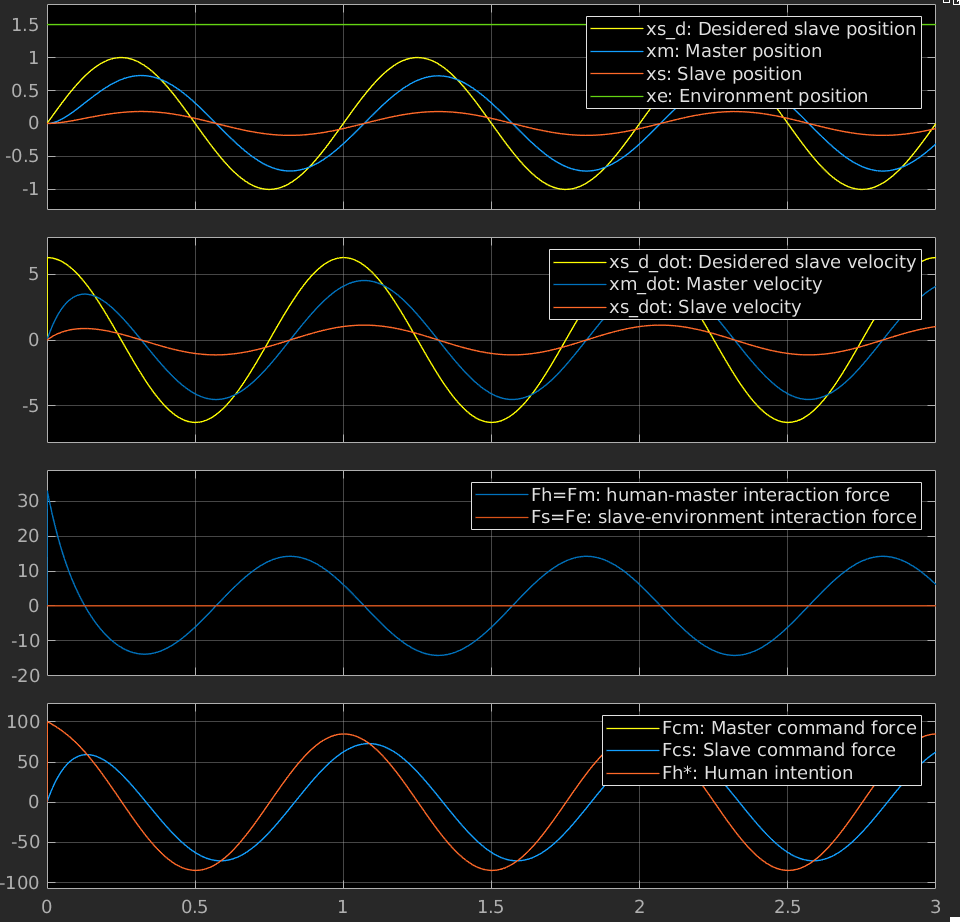
\includegraphics[keepaspectratio,width=\textwidth]{FF_free_nod}
\caption{2-channel F-F in free motion.}
\label{fig:ff_free}
\end{figure}
\begin{figure}[H]
\centering
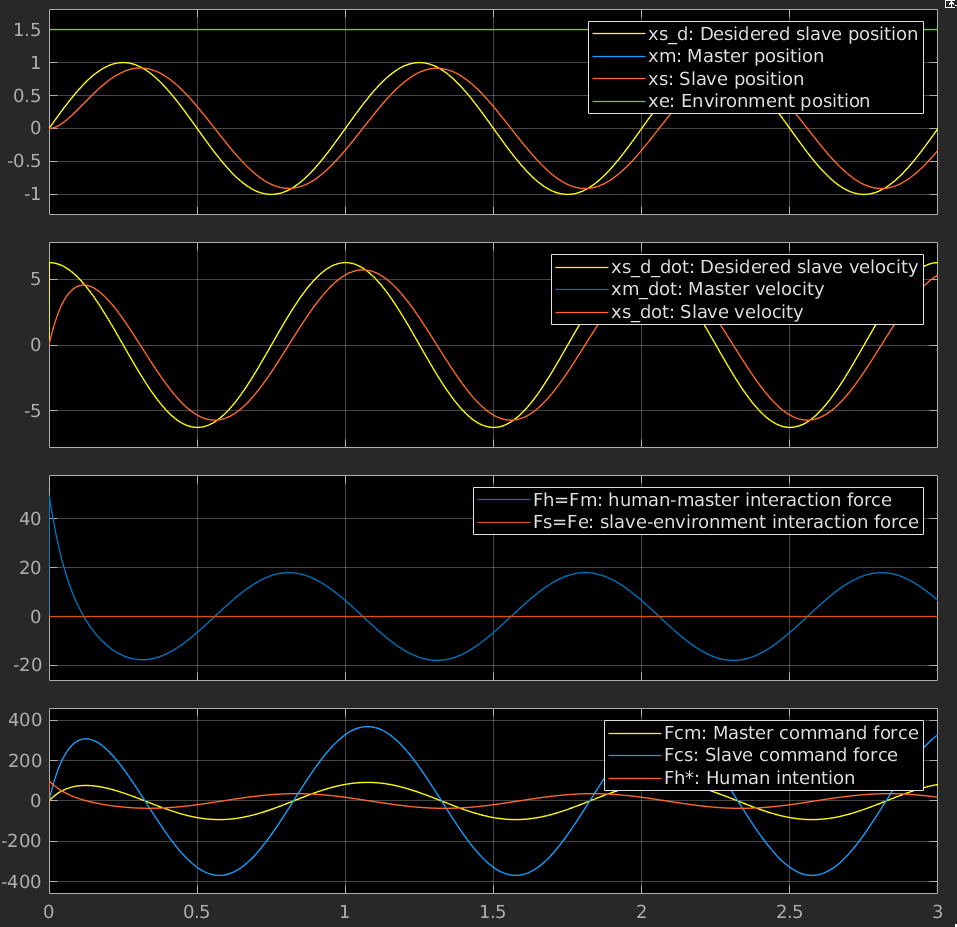
\includegraphics[keepaspectratio,width=\textwidth]{PFP_free_nod}
\caption{3-channel P,F-P in free motion.}
\label{fig:pfp_free}
\end{figure}
\end{minipage}
\end{figure}

\newpage

\begin{figure}[H]
\begin{minipage}{0.5\textwidth}
\begin{figure}[H]
\centering
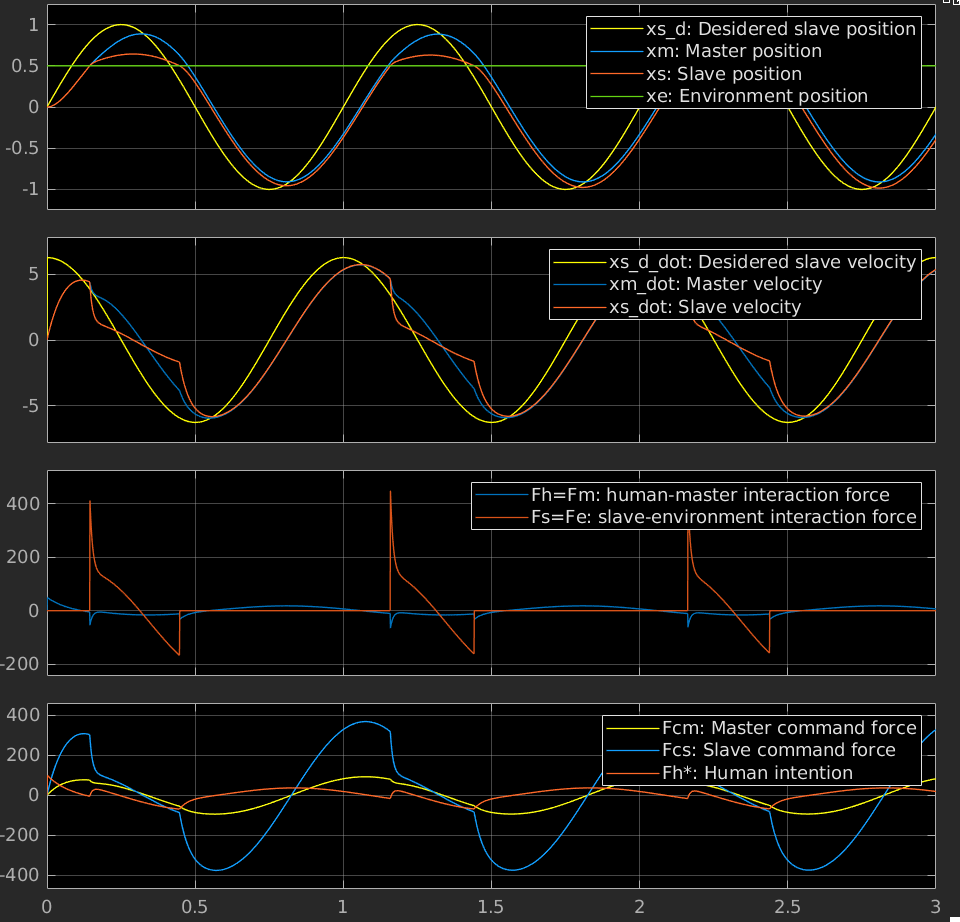
\includegraphics[keepaspectratio,width=\textwidth]{PP_contact_nod}
\caption{2-channel P-P in contact.}
\label{fig:pp_contact}
\end{figure}
\begin{figure}[H]
\centering
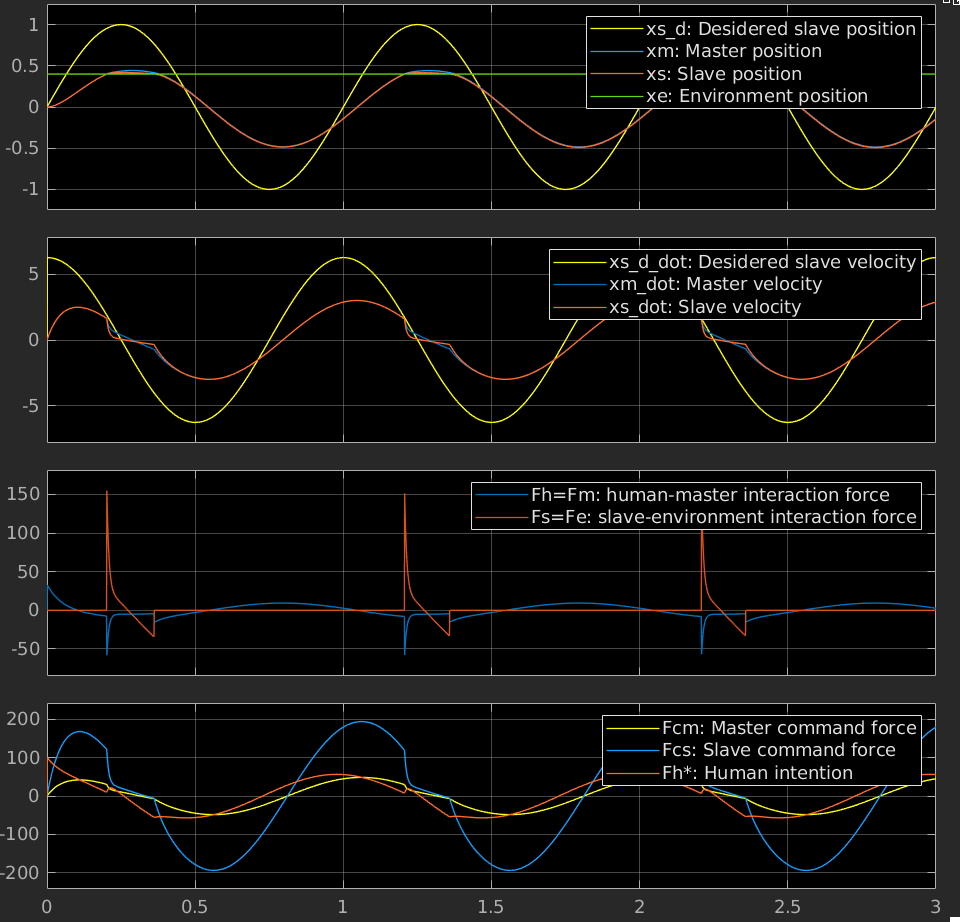
\includegraphics[keepaspectratio,width=\textwidth]{FP_contact_nod}
\caption{2-channel F-P in contact.}
\label{fig:fp_contact}
\end{figure}
\end{minipage}
\begin{minipage}{0.5\textwidth}
\begin{figure}[H]
\centering
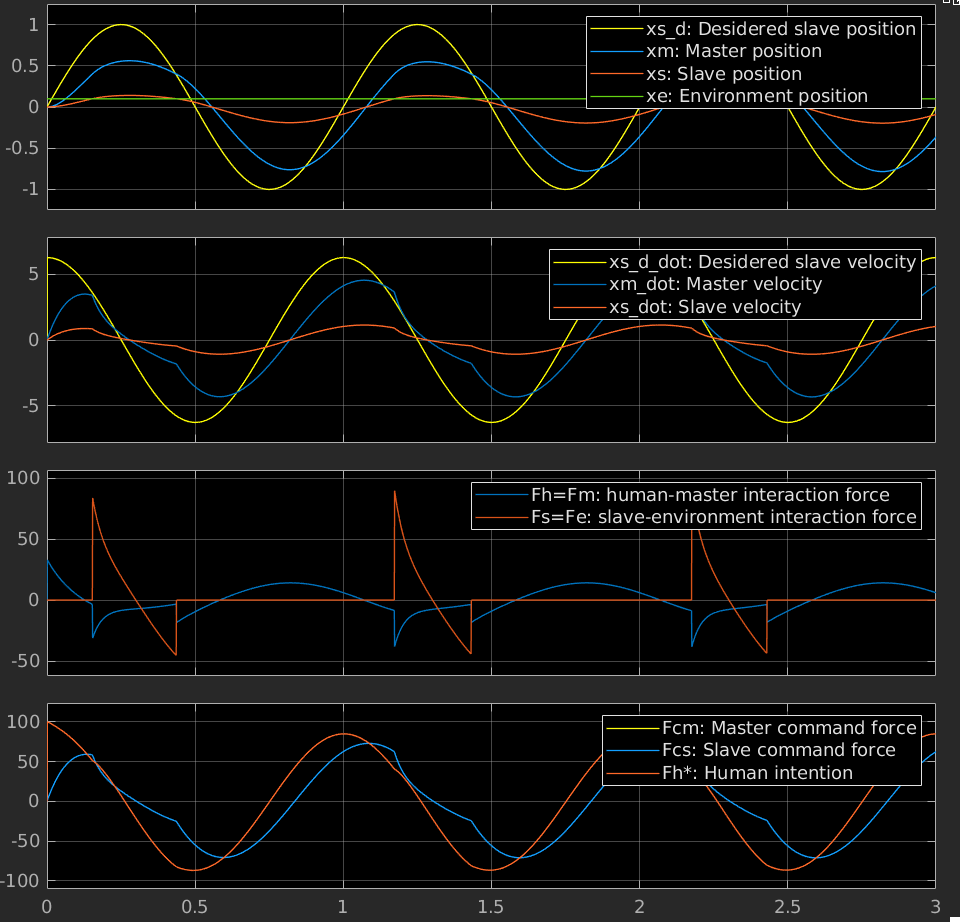
\includegraphics[keepaspectratio,width=\textwidth]{FF_contact_nod}
\caption{2-channel F-F in contact.}
\label{fig:ff_contact}
\end{figure}
\begin{figure}[H]
\centering
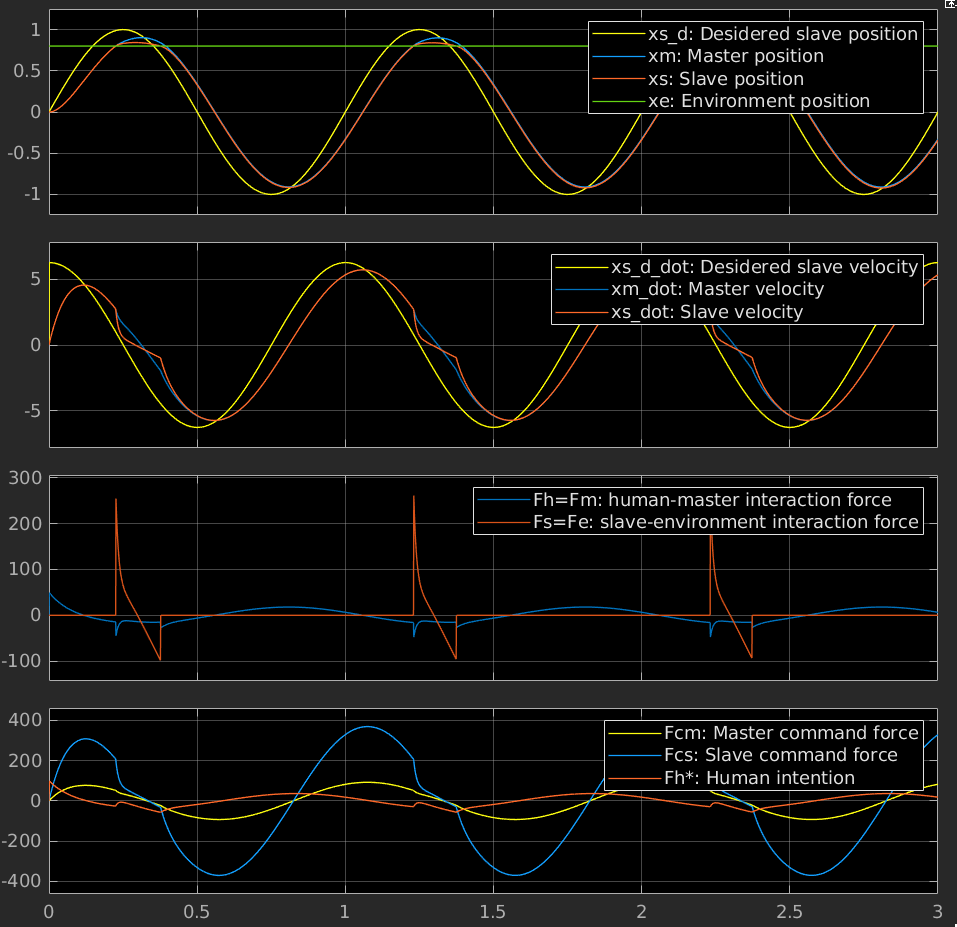
\includegraphics[keepaspectratio,width=\textwidth]{PFP_contact_nod}
\caption{3-channel P,F-P in contact.}
\label{fig:pfp_contact}
\end{figure}
\end{minipage}
\end{figure}

\newpage

\subsection{What happens if transportation delays are added in series to the coordinating controllers?}

\begin{figure}[H]
\begin{minipage}{0.5\textwidth}
\begin{figure}[H]
\centering
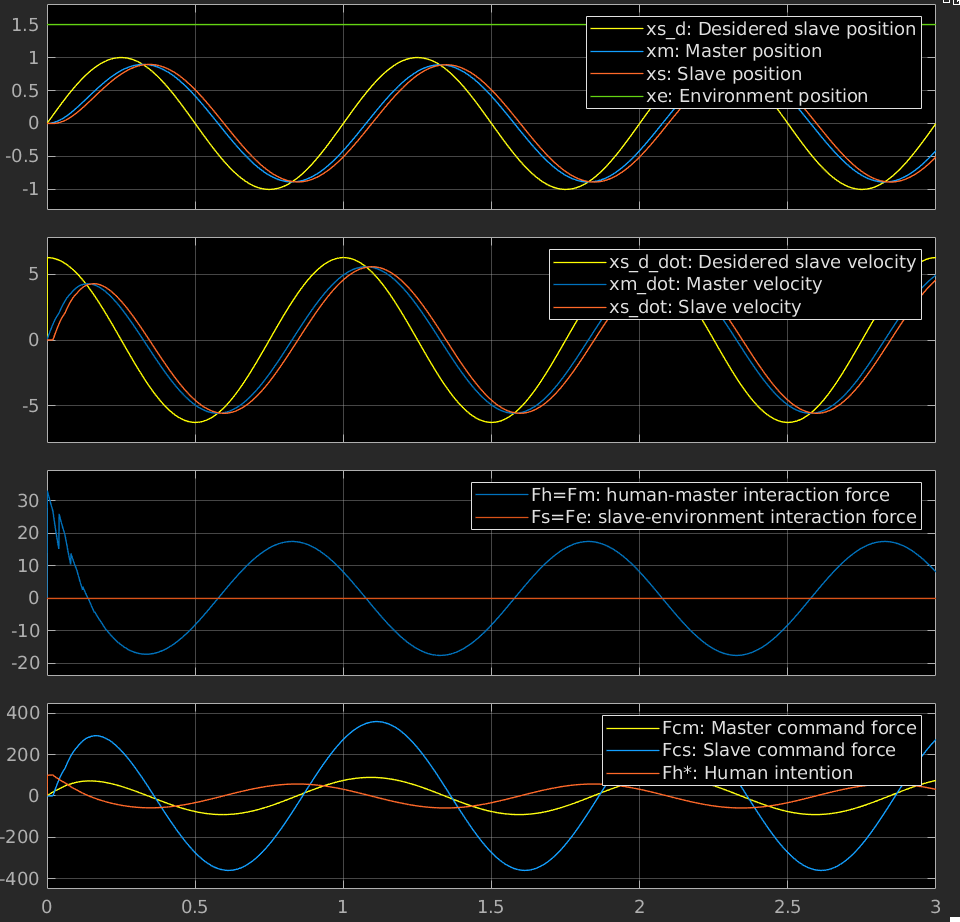
\includegraphics[keepaspectratio,width=\textwidth]{PP_d}
\caption{2-channel P-P in free motion with transportation delays.}
\label{fig:pp_d}
\end{figure}
\begin{figure}[H]
\centering
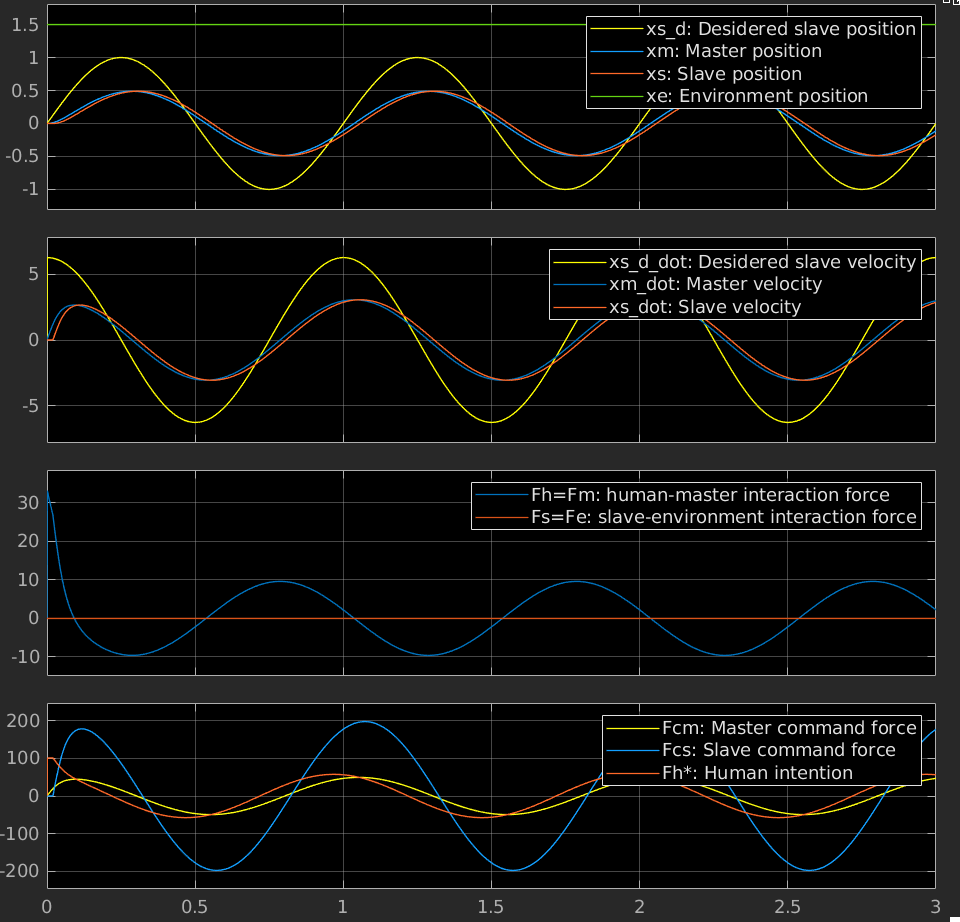
\includegraphics[keepaspectratio,width=\textwidth]{FP_d}
\caption{2-channel F-P in free motion with transportation delays.}
\label{fig:fp_d}
\end{figure}
\end{minipage}
\begin{minipage}{0.5\textwidth}
\begin{figure}[H]
\centering
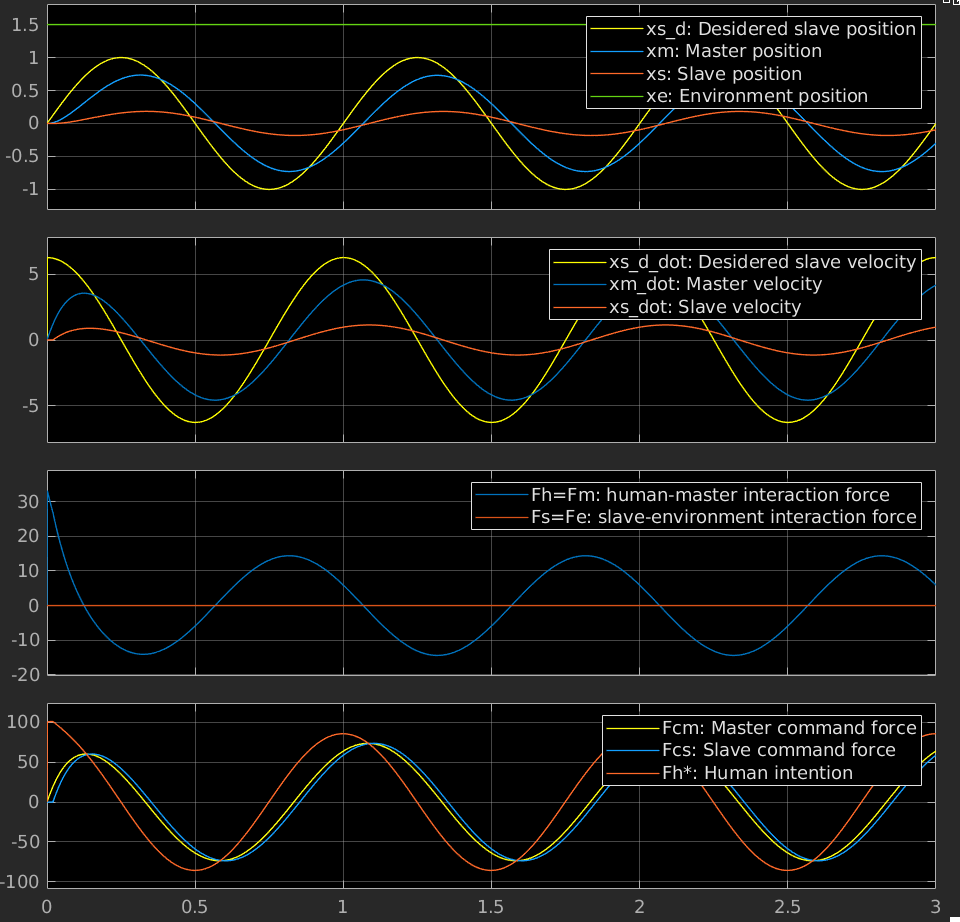
\includegraphics[keepaspectratio,width=\textwidth]{FF_d}
\caption{2-channel F-F in free motion with transportation delays.}
\label{fig:ff_d}
\end{figure}
\begin{figure}[H]
\centering
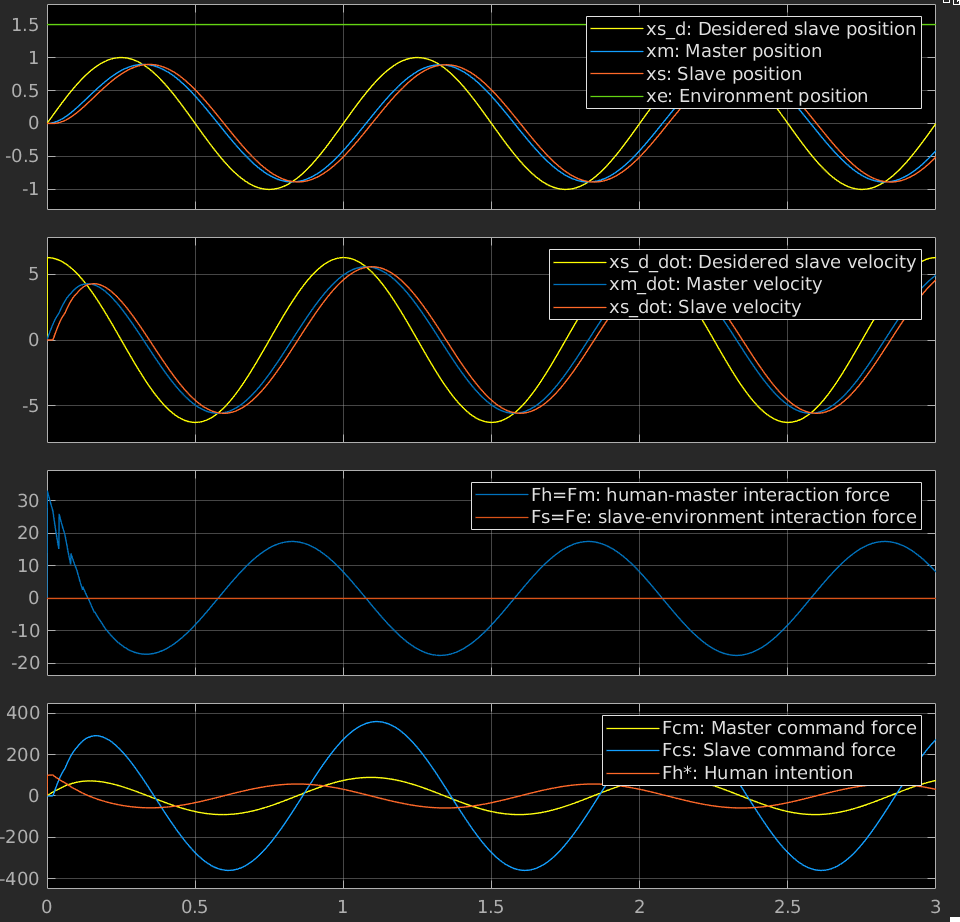
\includegraphics[keepaspectratio,width=\textwidth]{PFP_d}
\caption{3-channel P,F-P in free motion with transportation delays.}
\label{fig:pfp_d}
\end{figure}
\end{minipage}
\end{figure}

\newpage

\begin{figure}[H]
\begin{minipage}{0.5\textwidth}
\begin{figure}[H]
\centering
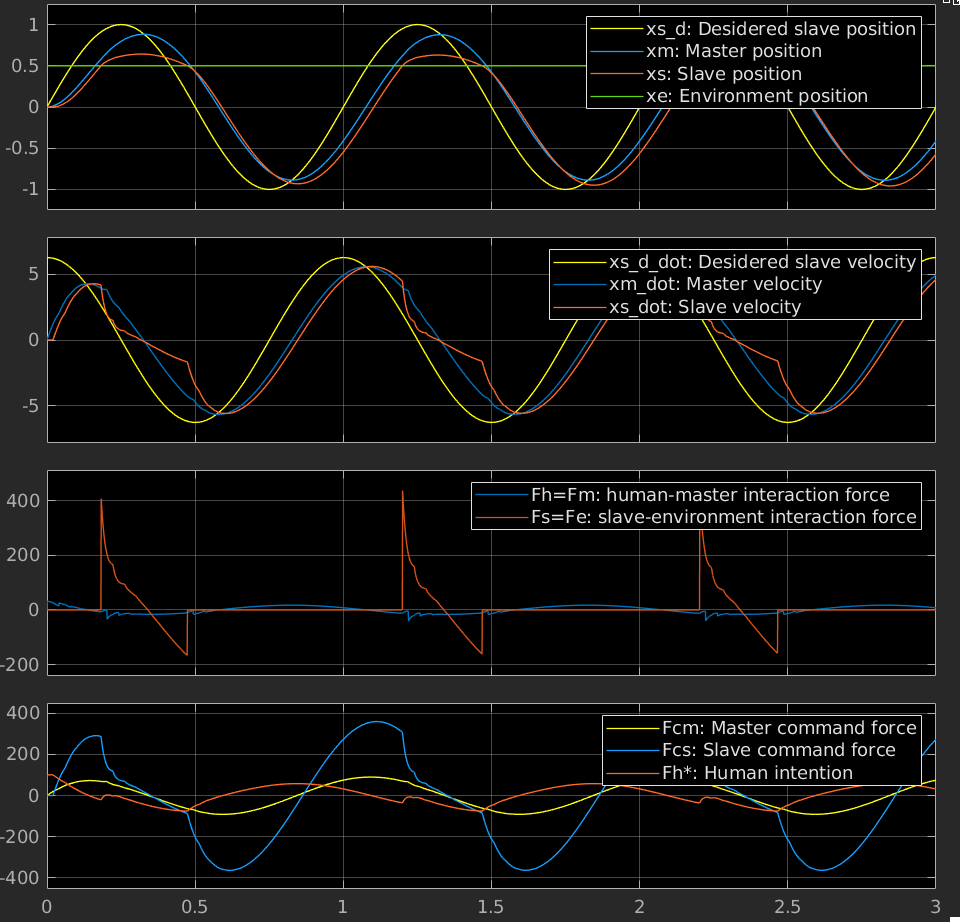
\includegraphics[keepaspectratio,width=\textwidth]{PP_contact_d}
\caption{2-channel P-P in contact with transportation delays.}
\label{fig:pp_contact_d}
\end{figure}
\begin{figure}[H]
\centering
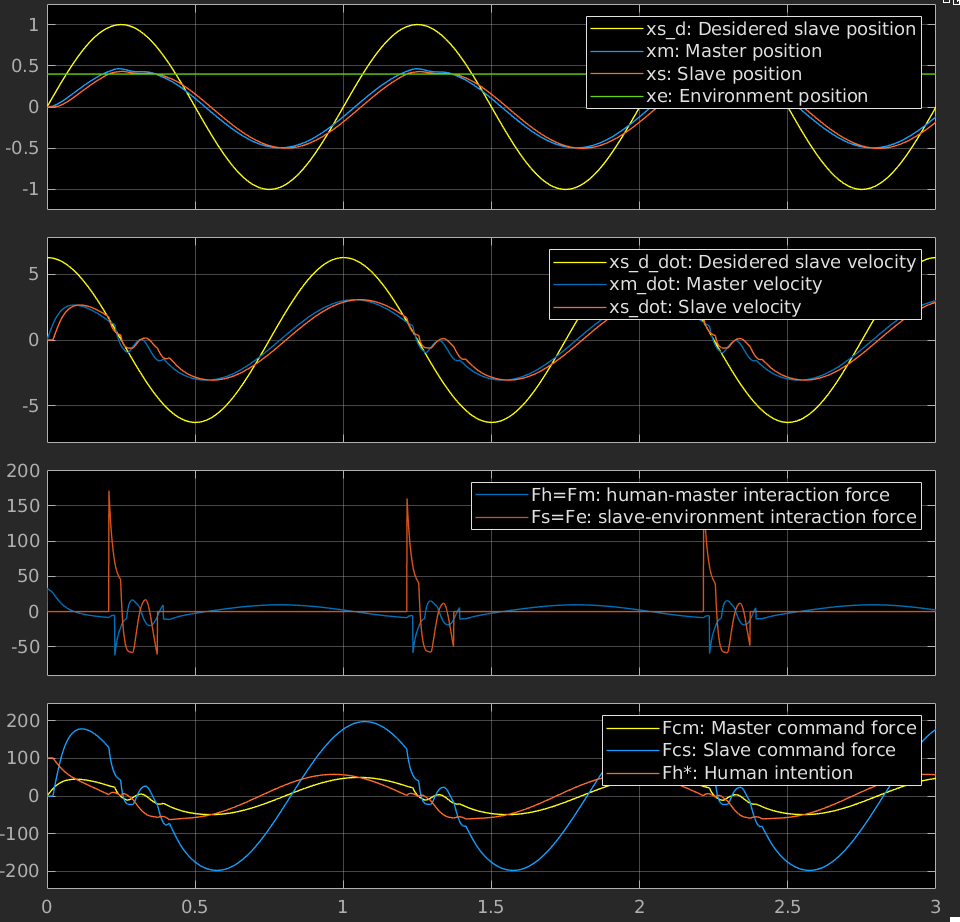
\includegraphics[keepaspectratio,width=\textwidth]{FP_contact_d}
\caption{2-channel F-P in contact with transportation delays.}
\label{fig:fp_contact_d}
\end{figure}
\end{minipage}
\begin{minipage}{0.5\textwidth}
\begin{figure}[H]
\centering
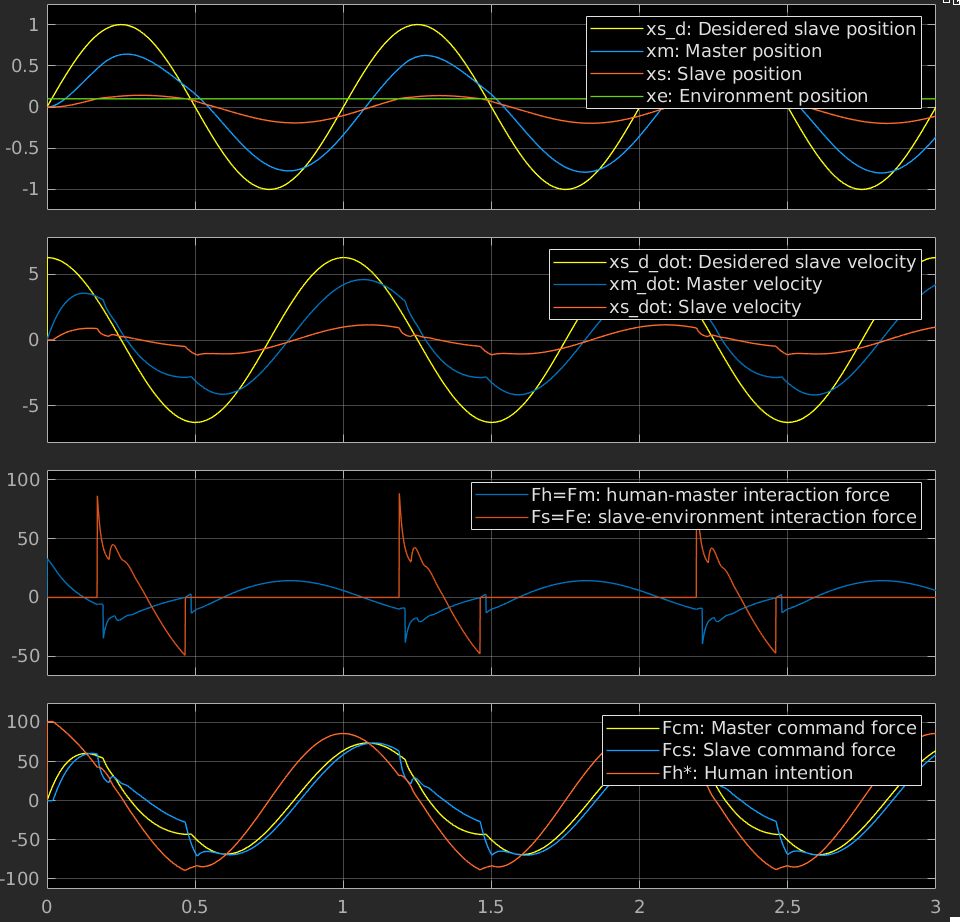
\includegraphics[keepaspectratio,width=\textwidth]{FF_contact_d}
\caption{2-channel F-F in contact with transportation delays.}
\label{fig:ff_contact_d}
\end{figure}
\begin{figure}[H]
\centering
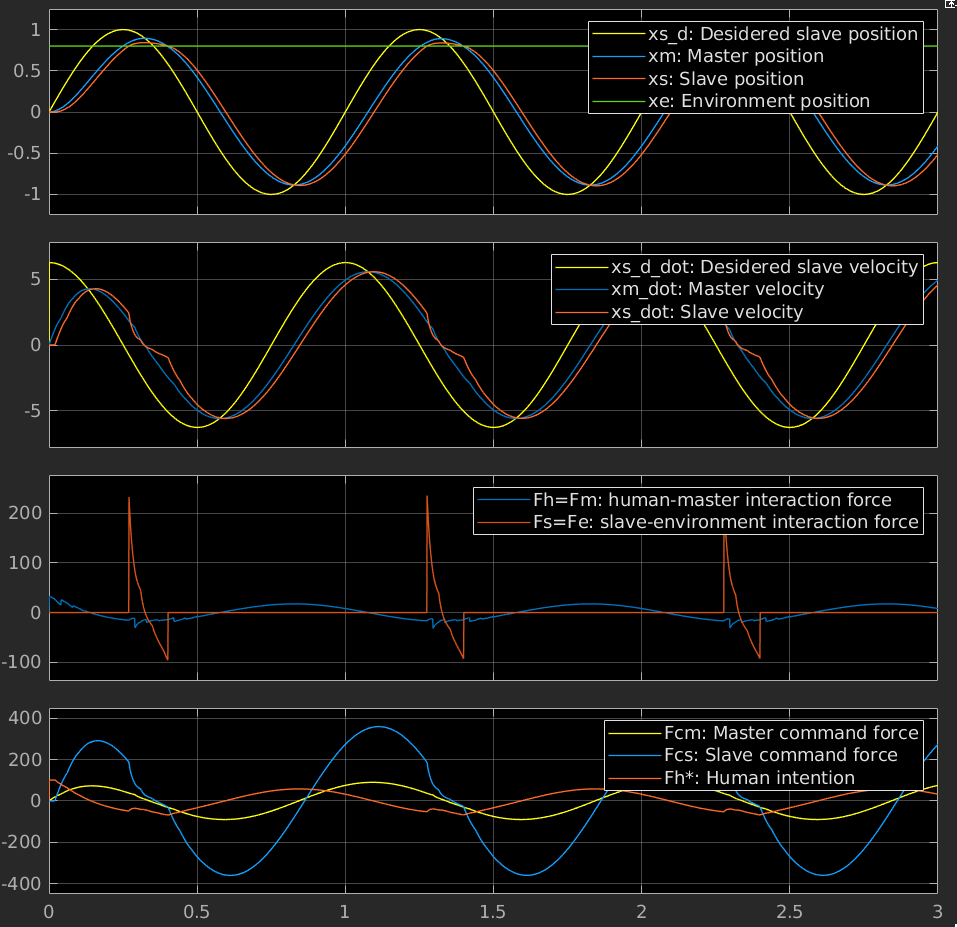
\includegraphics[keepaspectratio,width=\textwidth]{PFP_contact_d}
\caption{3-channel P,F-P in contact with transportation delays.}
\label{fig:pfp_contact_d}
\end{figure}
\end{minipage}
\end{figure}

\newpage

\section{Assignment 3}
\label{ass3}
\subsection{Implement the Kalman filter/predictor and estimate the velocity and acceleration from noisy position measurements}

Both the Kalman filter and the Kalman predictor are based on the stochastic LTI system:

\begin{equation*}
\begin{cases}
\textbf{x}_{k+1}=A\textbf{x}_k+Bw_k\\
y_k=C\textbf{x}_k+v_k
\end{cases}\;\;\;\;\textbf{x}=\begin{bmatrix}
x\\\dot x\\\ddot x
\end{bmatrix}\;\;\;
A=\begin{bmatrix}
1 & T_s & \frac{T_s^2}{2}\\
0 & 1 & T_s\\
0 & 0 & 1
\end{bmatrix}\;\;\; B=\begin{bmatrix}
\frac{T_s^3}{6}\\\frac{T_2}{2}\\T_s
\end{bmatrix}\;\;\; C=\begin{bmatrix}
1 & 0 & 0
\end{bmatrix}
\end{equation*}

and $w_k$, $v_k$ zero mean uncorrelated Gaussian random variables describing respectively model and noise variances:

\begin{equation*}
w_k=\mathcal N(0,Q)\;\;\;\;v_k=\mathcal N(0,R)
\end{equation*}

with $Q=qBB^T$, $R=var(x)$, $q=10^7$ and initial state $x_0\approx\mathcal N(\bar x_0,P_0)$, $\bar x_0=\begin{bmatrix}
0 & 0 & 0
\end{bmatrix}^T, P_0=\mathbb{I}_3\cdot 1\cdot 10^{-5}$.

The Kalman filter is recursively defined as follows:
\begin{align*}
\hat x_{k+1\mid k+1}&=A\hat x_{k\mid k}+K_{k+1}(y_{k+1}-CA\hat x_{k\mid k})\\
P_{k+1\mid k}&=AP_{k\mid k-1}A^T-AP_{k\mid k-1}C^T(CP_{k\mid k-1}C^T+R)^{-1}CP_{k\mid k-1}A^T+Q
\end{align*}

where $P$ is the variance of the estimation error and the Kalman gain (the matrix that maps the output estimation error into the correction of the state) defined as:
\begin{equation*}
K_{k+1}=P_{k+1\mid k}C^T(CP_{k+1\mid k}C^T+R)^{-1}
\end{equation*}

The Kalman predictor is recursively defined as follows:
\begin{align*}
\hat x_{k+1\mid k}&=A\hat x_{k\mid k-1}+\bar K_{k}(y_{k}-C\hat x_{k\mid k-1})\\
P_{k+1\mid k}&=AP_{k\mid k-1}A^T-AP_{k\mid k-1}C^T(CP_{k\mid k-1}C^T+R)^{-1}CP_{k\mid k-1}A^T+Q
\end{align*}

with the Kalman gain defined as:
\begin{equation*}
\bar K_{k}=AP_{k\mid k-1}C^T(CP_{k\mid k-1}C^T+R)^{-1}
\end{equation*}

The difference between filter and predictor is that the former estimates the state $\hat x$ at time $k+1$ given measurements until time $k+1$, while the latter estimates the state $\hat x$ at time $k+1$ given measurements until time $k$ (1-step ahead prediction). Therefore the resulting estimations will differ only in the first state. Both filter and predictor are applied to a position signal with Gaussian noise and a signal with quantization noise. The results are shown in figures \ref{fig:kalman_fp_gauss} and \ref{fig:kalman_fp_quant}.

\subsection{Implement the steady-state Kalman filter/predictor and estimate the velocity and acceleration from noisy position measurements}

The steady state Kalman filter and predictor are obtained by computing a fixed solution for the estimation error variance $P_{\infty}$ and for the Kalman gain, $K_{\infty}$. The estimation error variance for $k\to\infty$ is obtained by solving the Algebraic Riccati Equation:

\begin{equation*}
P_\infty = AP_\infty A^T-AP_\infty C^T(CP_\infty C^T + R)^{-1}CP_\infty A^T + Q
\end{equation*}

Then, the Kalman gains for the filter and predictor are defined as:

\begin{equation*}
K_\infty = P_\infty C^T(CP_\infty C^T+R)^{-1}\;\;\;\;\bar K_\infty = AP_\infty C^T(CP_\infty C^T+R)^{-1}
\end{equation*}

Finally, the steady state Kalman filter is defined as:

\begin{equation*}
\hat x_{k+1\mid k+1}=A\hat x_{k\mid k}+K_\infty(y_{k+1}-CA\hat x_{k\mid k})
\end{equation*}

while the steady state Kalman predictor is defined as:

\begin{equation*}
\hat x_{k+1\mid k}=A\hat x_{k\mid k-1}+\bar K_\infty(y_{k}-C\hat x_{k\mid k-1})
\end{equation*}

Both filter and predictor are applied to a position signal with Gaussian noise and a signal with quantization noise. The results are shown in figures \ref{fig:kalman_fp_gauss} and \ref{fig:kalman_fp_quant}.

\begin{figure}[H]
\centering
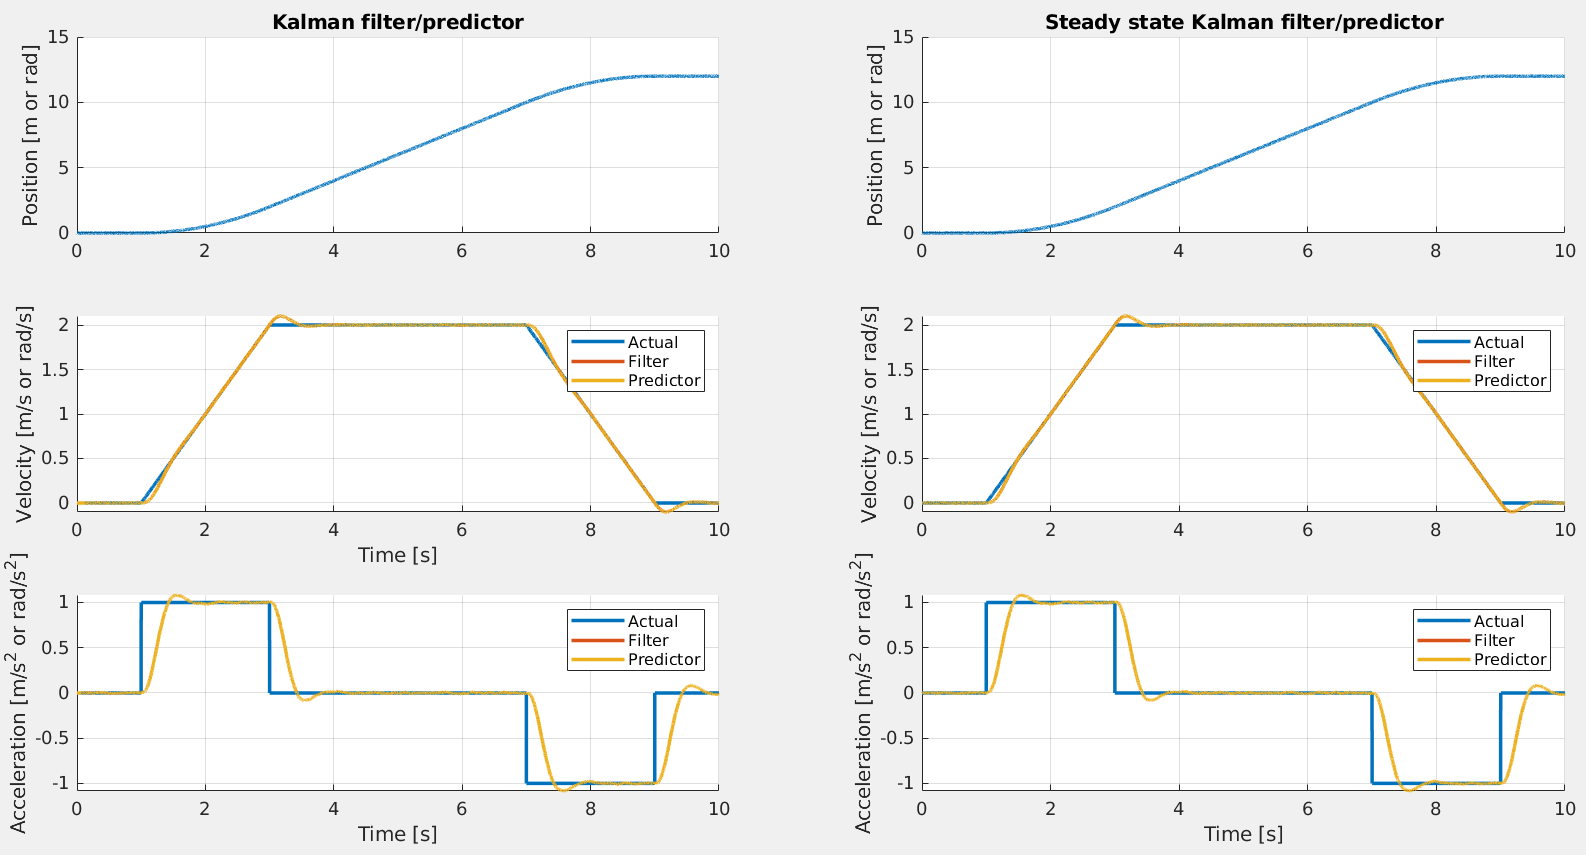
\includegraphics[keepaspectratio,width=\textwidth]{kalman_fp_gauss}
\caption{Kalman filter/predictor applied to a position signal with Gaussian noise}
\label{fig:kalman_fp_gauss}
\end{figure}

\begin{figure}[H]
\centering
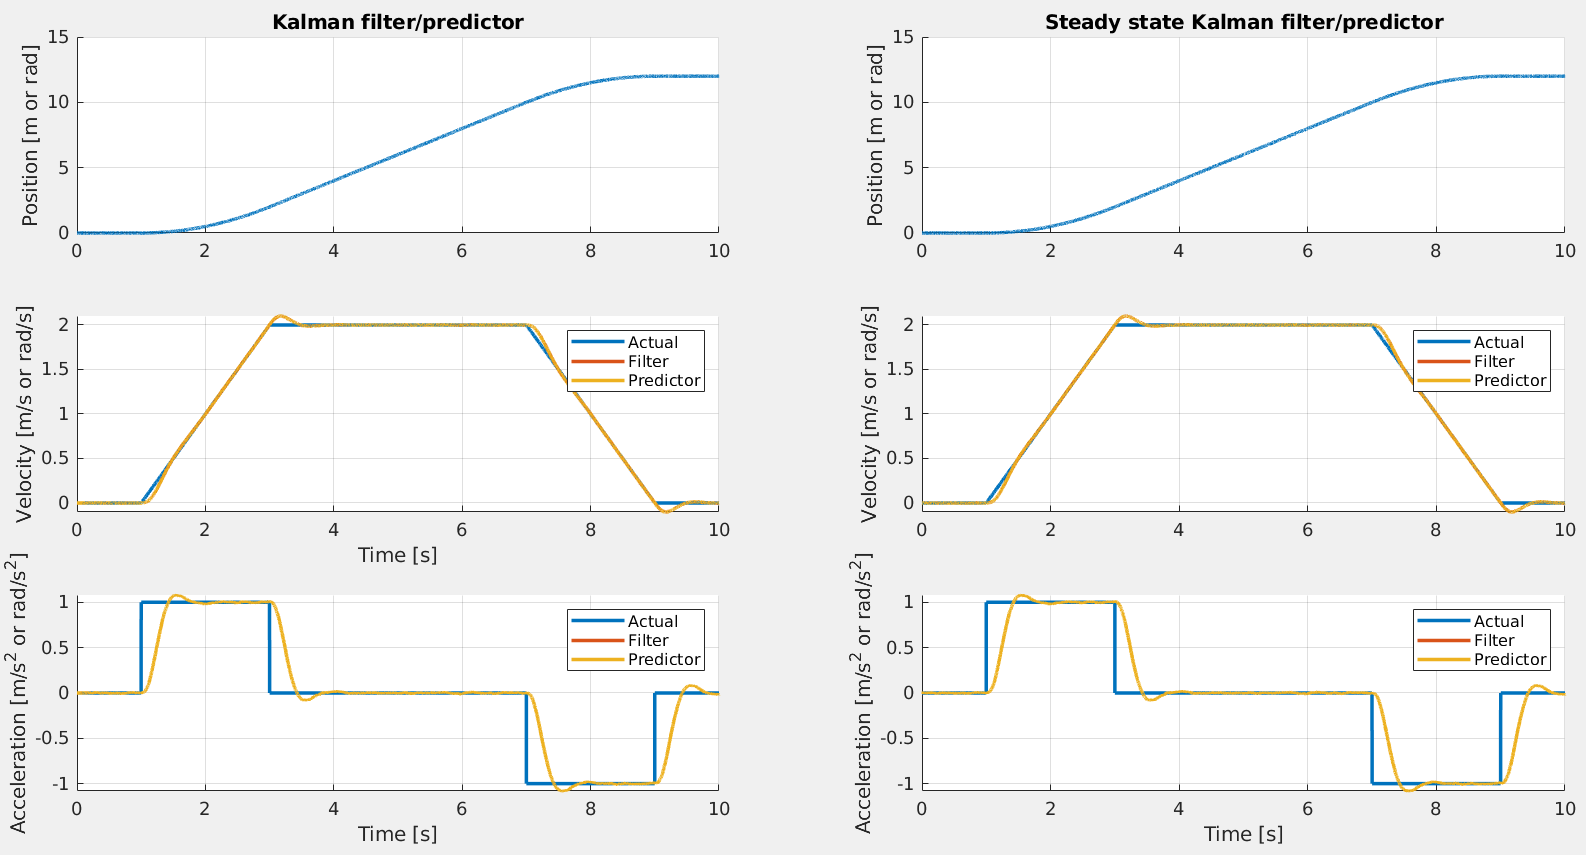
\includegraphics[keepaspectratio,width=\textwidth]{kalman_fp_quant}
\caption{Kalman filter/predictor applied to a position signal with quantization noise}
\label{fig:kalman_fp_quant}
\end{figure}

As expected, both filter and predictor produce the same estimations, and there's no difference with their respective steady-state implementations. Both the Gaussian and quantization noise cases produce very similar estimates.

\newpage

\section{Assignment 4}

\subsection{Implement the Kalman smoother and estimate the velocity and acceleration from noisy position measurements}

Starting with the same model described in assignment \ref{ass3}, the Kalman smoother is defined in two parts. a forward step consisting of standard Kalman filtering and a backward step in which the smoothing takes place.

In the forward step, a standard Kalman filtering procedure is carried out:
\begin{align*}
\hat x_{k+1\mid k+1}^f &= A\hat x_{k\mid k}^f +K_{k+1}(y_{k+1}-CA\hat x_{k\mid k}^f)\\
\hat x_{0\mid 0}^f&=\bar x_0\\
P_{0\mid 0}^f &= P_0\\
P_{k\mid k}^f &= P_{k-1\mid k-1}^f - KCP_{k-1\mid k-1}^f\\
P_{k+1\mid k}^f &= AP_{k\mid k}^fA^T + Q 
\end{align*}

Then in the backward step, smoothing is carried out as follows:
\begin{align*}
\hat x_{k\mid N}^s&=\hat x_{k\mid k}^f+\breve K_k(\hat x_{k+1\mid N}^s-\hat x_{k+1\mid k}^f)\\
\hat x_{N\mid N}^s&=\hat x_{N\mid N}^f
\end{align*}

where:
\begin{equation*}
\breve K_k = P_{k\mid k}^fA^T(P_{k+1\mid k}^f)
\end{equation*}

and the conditional covariance matrix $P_{k\mid N}$ satisfies:
\begin{align*}
P_{k\mid N}&=P_{k\mid k}^f+\breve K-k(P_{k+1\mid N}-P_{k+1\mid k}^f)\\
P_{N\mid N} &= P_{N\mid N}^fs
\end{align*}

The smoother is applied to a position signal with Gaussian noise and a signal with quantization noise, and compared to the estimation given by the Kalman filter. The results are shown in figures \ref{fig:kalman_s_gauss} and \ref{fig:kalman_s_quant}.


\begin{figure}[H]
\centering
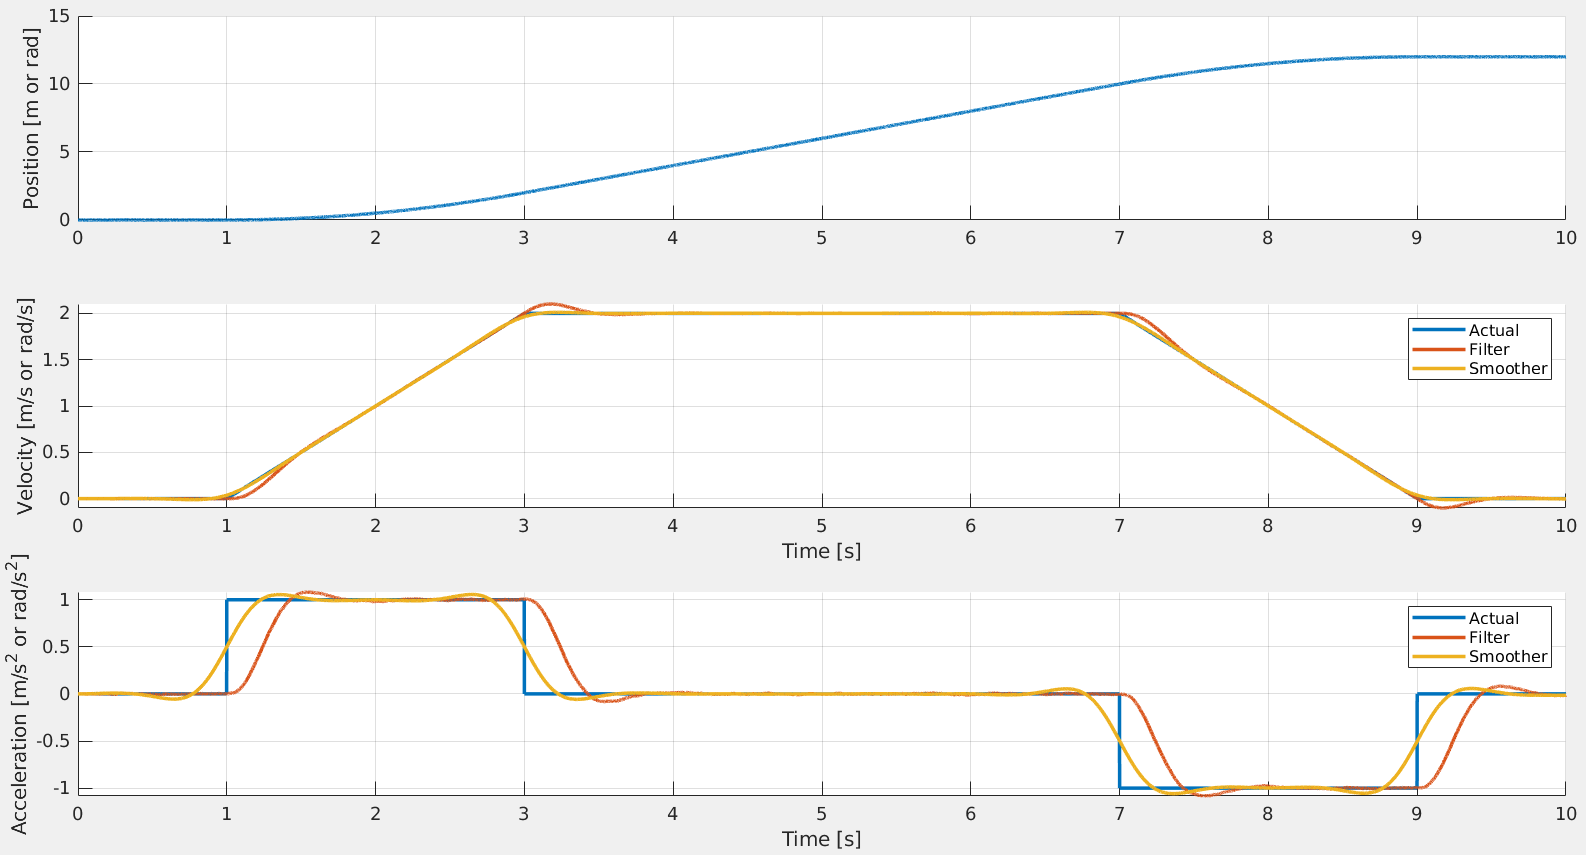
\includegraphics[keepaspectratio,width=\textwidth]{kalman_s_gauss}
\caption{Kalman smoother vs Kalman filter applied to a position signal with Gaussian noise}
\label{fig:kalman_s_gauss}
\end{figure}

\begin{figure}[H]
\centering
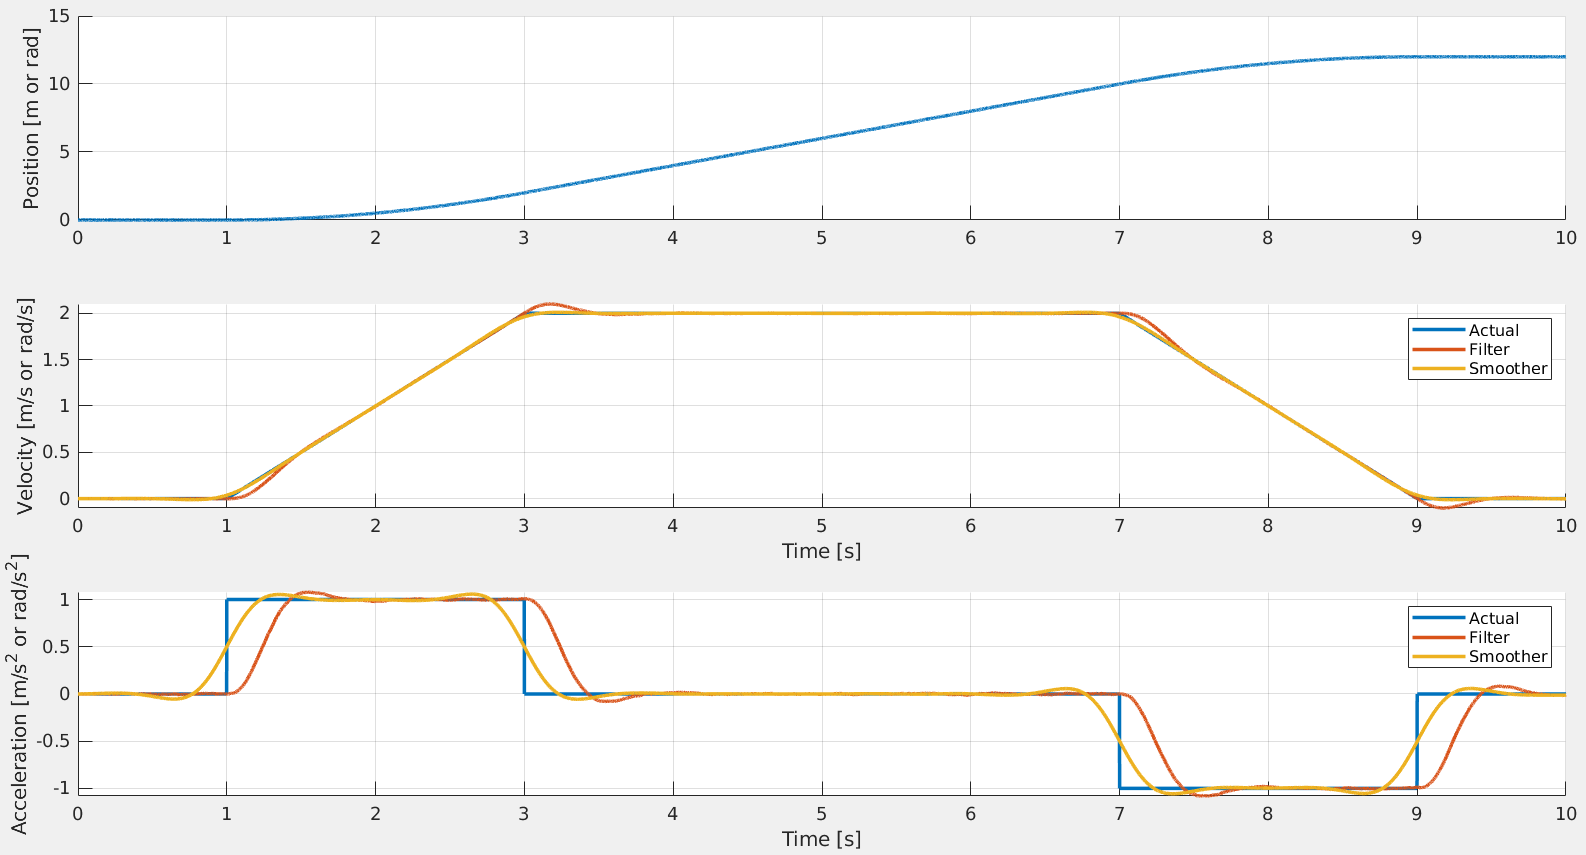
\includegraphics[keepaspectratio,width=\textwidth]{kalman_s_quant}
\caption{Kalman smoother vs Kalman filter applied to a position signal with quantization noise}
\label{fig:kalman_s_quant}
\end{figure}

The smoother effectively improves the estimation of the velocity, especially near the discontinuity points, and of the acceleration, making the shape of the estimation more closely match the "actual" acceleration.

\newpage

\section{Assignment 5}

\subsection{Identify the parameters J and D using the LS and the RLS on the DC motors data}

DC motors are characterized by the differential equation:
\begin{equation*}
\tau\dot\omega(t)+\omega(t)=kV(t)
\end{equation*}

that links the applied voltage $V(t)$ to the angular velocity and acceleration of the motor $\omega(t),\dot\omega(t)$ through the constants $k$ and $\tau$. $\tau$ is related to the motor's inertia, while $k$ is related to the motor's torque and electrical constants.

Assuming the motor model is linear, we can estimate $k$ and $\tau$ using Least Squares (LS) regression, which is a method that estimates the vector $\hat\beta$ of parameters that best explains the relation between a set of input vectors $X\in\R^{N\times m}$ to a set of output vectors $Y\in\R^{N\times 1}$. $\hat\beta$ is the parameter vector that minimizes the residual sum of squares (RSS):
\begin{equation*}
\hat\beta = \underset{\beta}{argmin}RSS(\beta)=\underset{\beta}{argmin}(Y-X\beta)^T(Y-X\beta)
\end{equation*}

If $X^TX$ is nonsingular there exists an unique solution given by the normal equations:
\begin{equation*}
\grad_\beta RSS(\beta)=0\iff X^T(Y_X\beta)=0\implies\hat\beta=(X^TX)^{-1}X^TY
\end{equation*}

By expanding the inner products between the vector sets into the sum of the inner products of the vectors that make up the sets and exploiting the matrix inversion lemma to get rid of the matrix inversion, a recursive solution for $\hat\beta$ can be found as:
\begin{align*}
\hat\beta(k)&=\hat\beta(k-1)+K(k)e(k)\;\;\;\;\text{with }\begin{cases}
K(k)&=P(k)x_k^T\\
e(k)&=y_k-x_k\hat\beta(k-1)\\
P(k)&=\frac{1}{\lambda}\left[P(k-1)-\frac{P(k-1)x_k^Tx_kP(k-1)}{\lambda+x_kP(k-1)x_k^T}\right]\end{cases}
\end{align*}

where $\lambda$ is a parameter called forgetting factor which increases the weight of the correction applied to $\hat\beta$ for the most recent samples, which is useful to improve the estimation for time-varying quantities.

Both methods were implemented and tested on data collected from a DC motor modelled in SIMULINK. The $X$ vector set is made up of a set of angular accelerations and velocities obtained by applying a Kalman smoother to the angular position data measured by an encoder, while the $Y$ vector set is made up of the corresponding command voltages. The parameter vector is $\hat\beta=\begin{bmatrix}
k\tau & 1/k
\end{bmatrix}$. LS results are $k=0.7036,\tau=0.2542$ while RLS (with $\lambda=0.975$) results are $k=0.0174,\tau=0.0642$. The corresponding $\hat\beta$ vectors were used to reproject the samples $X$ to obtain an estimation for the voltages $Y$. Figure \ref{fig:ls} shows the resulting estimates against the ground truth.

\begin{figure}[H]
\centering
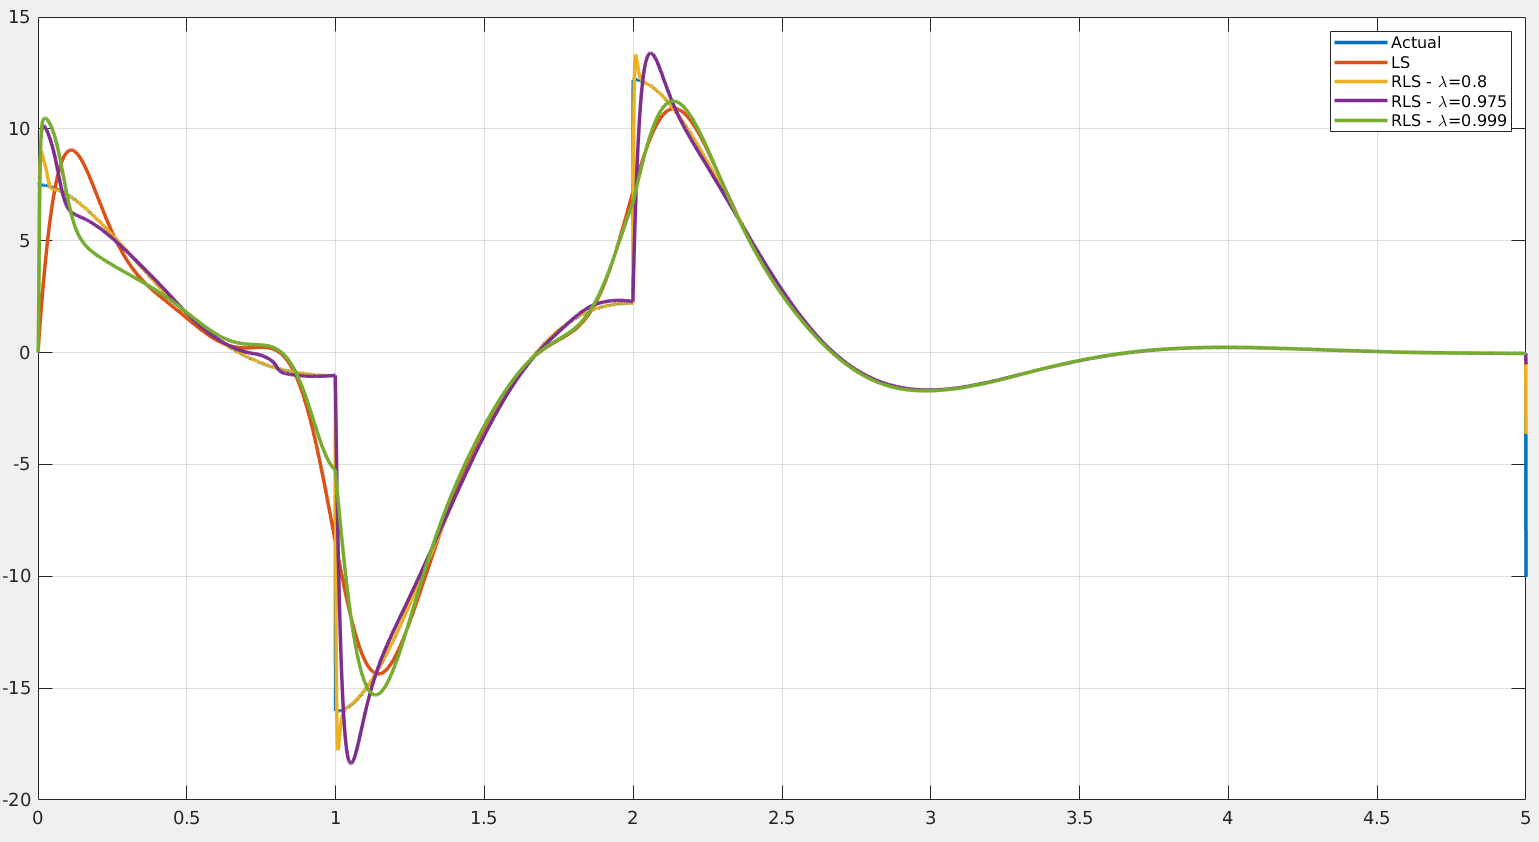
\includegraphics[keepaspectratio,width=0.75\textwidth]{ls}
\caption{Comparison of actual and reprojected voltages}
\label{fig:ls}
\end{figure}

LS performs reasonably well, matching the actual voltages most of the time, but RLS improves greatly the estimation especially around the discontinuities in the actual voltages, showing its capability of accurately tracking time-varying quantities.
Decreasing the value of $\lambda$ results in a model with smaller variance but increased bias towards the ground truth, while increasing it reduces the bias towards the ground truth and increases the variance.

\newpage

\section{Assignment 6}

\subsection{Implement the Scattering-based bilateral teleoperation architecture for the F-P and P-P cases}

\begin{figure}[h]
\centering
\includegraphics[keepaspectratio,width=\textwidth]{scattering_fp}
\caption{Scattering-based F-P teleoperation architecture}
\end{figure}

\begin{figure}[h]
\centering
\includegraphics[keepaspectratio,width=\textwidth]{scattering_pp}
\caption{Scattering-based P-P teleoperation architecture}
\end{figure}

Passivity, and therefore stability, is introduced by using wave variables in the communication channel. The scattering operation in the FP case is defined as:

\begin{equation*}
\begin{cases}
u_m=\sqrt{2b}\dot x_m+v_m\\
f_m=b\dot x_m + \sqrt{2b}v_m
\end{cases}\;\;\;\;\;\;\begin{cases}
u_s = \sqrt{\frac{2}{b}}f_s-v_s\\
\dot x_s= -\frac{1}{b}(f_s-\sqrt{2b}v_s)
\end{cases}
\end{equation*}

while in the PP case is defined as:

\begin{equation*}
\begin{cases}
u_m=\sqrt{\frac{2}{b}}\dot f_m-v_m\\
\dot x_m=\frac{1}{b} (f_m - \sqrt{2b}v_m)
\end{cases}\;\;\;\;\;\;\begin{cases}
u_s = \sqrt{\frac{2}{b}}f_s-v_s\\
\dot x_s= -\frac{1}{b}(f_s-\sqrt{2b}v_s)
\end{cases}
\end{equation*}

Between the wave variables, a 10 time-step delay and a low pass filter with a $5Hz$ cutoff frequency are introduced. The presence of the delay does not affect the stability of the system.

\newpage

\subsection{Compare positions, velocities, forces, commands in free motion and in contact}

\begin{figure}[H]
\begin{minipage}{0.5\textwidth}
\centering
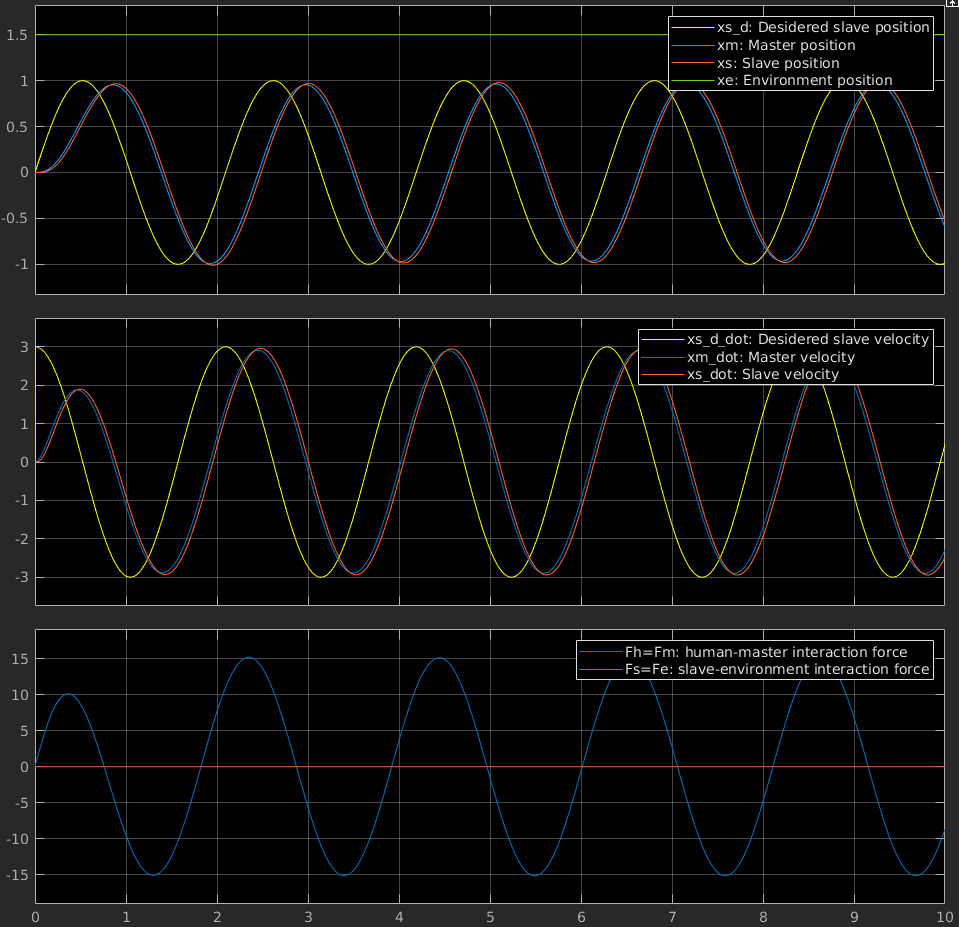
\includegraphics[keepaspectratio,width=\textwidth]{sfp_free_nok}
\caption{FP in free motion, without noise}
\label{fig:sfp_free_nok}

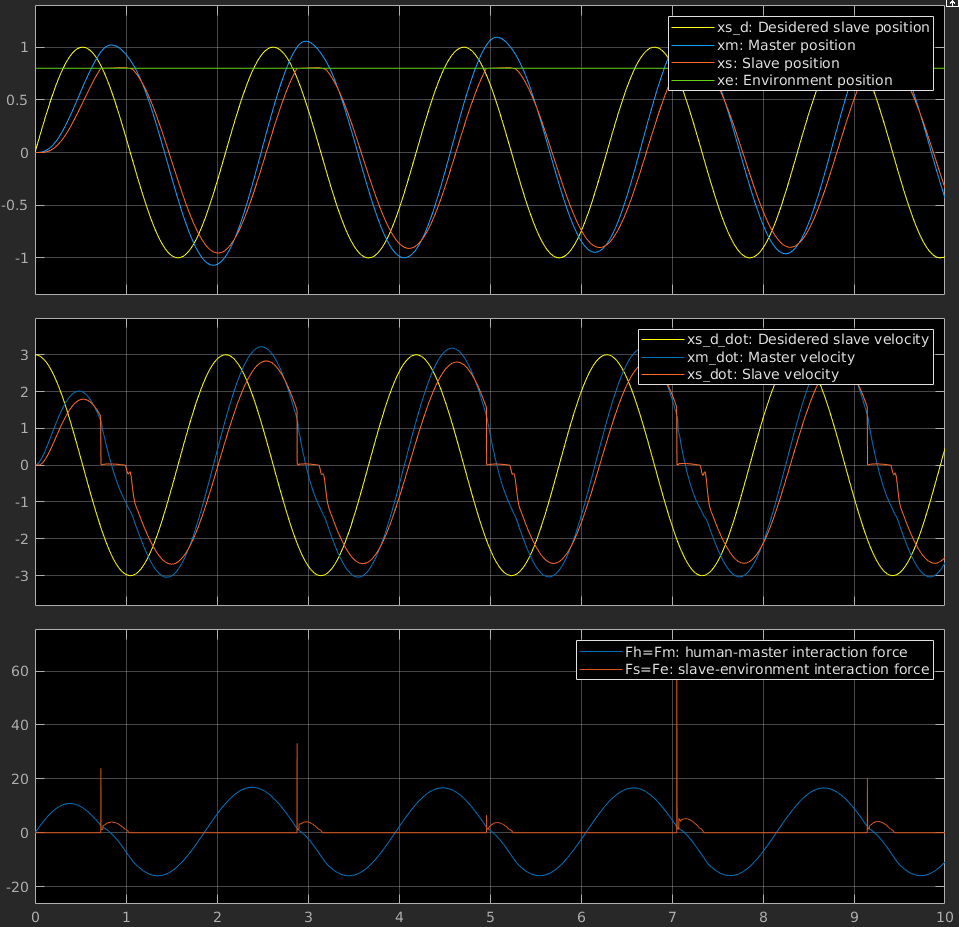
\includegraphics[keepaspectratio,width=\textwidth]{sfp_contact_nok}
\caption{FP in contact, without noise}
\label{fig:sfp_contact_nok}
\end{minipage}
\begin{minipage}{0.5\textwidth}
\centering
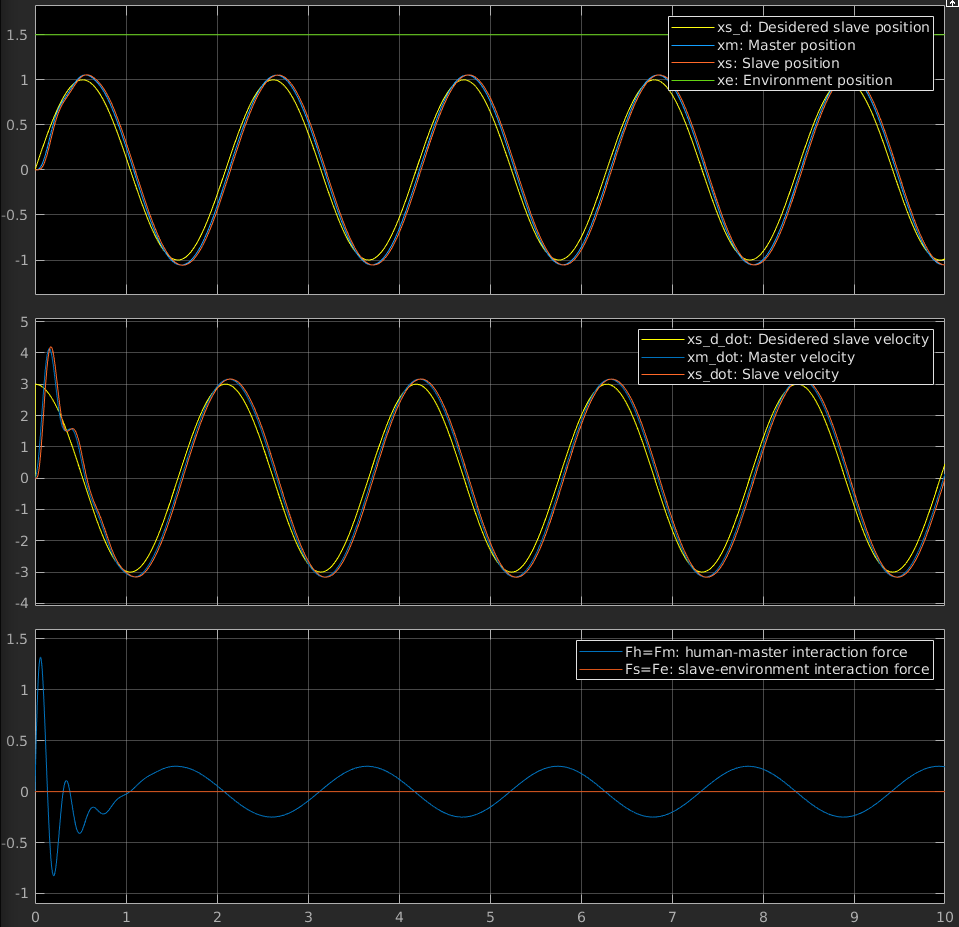
\includegraphics[keepaspectratio,width=\textwidth]{spp_free_nok}
\caption{PP in free motion, without noise}
\label{fig:spp_free_nok}

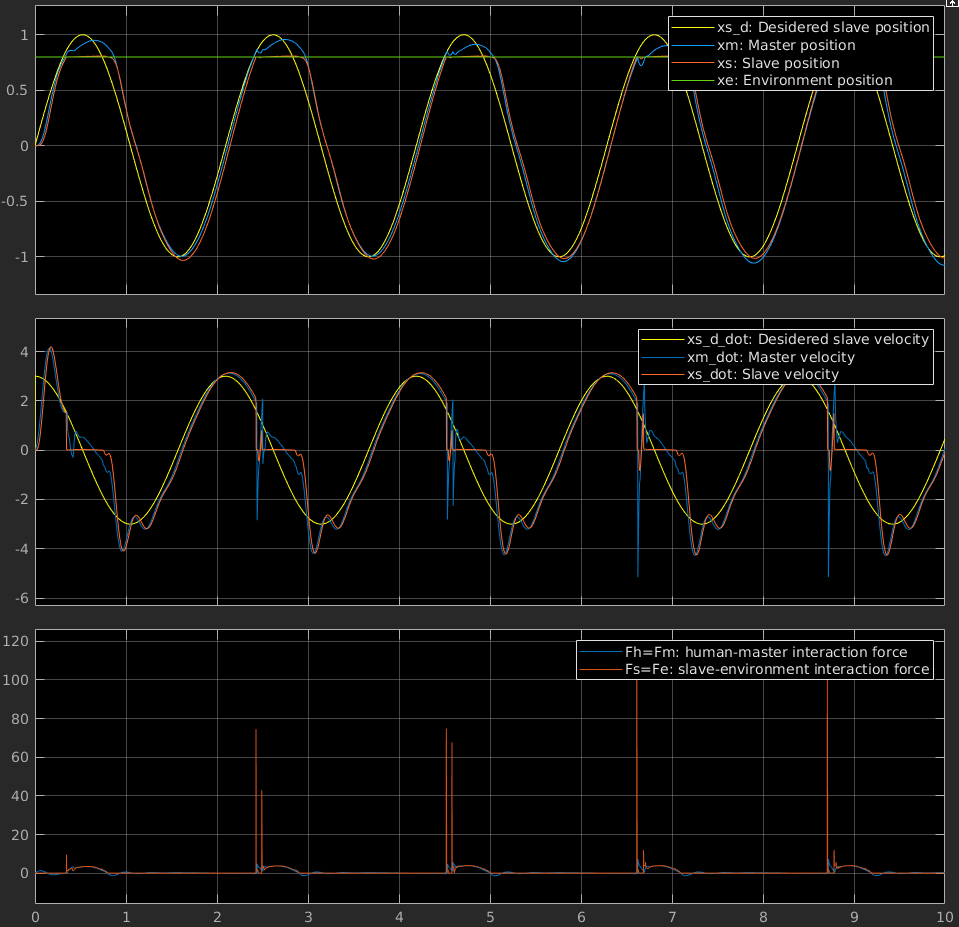
\includegraphics[keepaspectratio,width=\textwidth]{spp_contact_nok}
\caption{PP in contact, without noise}
\label{fig:spp_contact_nok}
\end{minipage}
\end{figure}

\newpage

\subsection{Create another simulink model and (a) add the measurement noise to the position/force signals, and (b) estimate velocities from positions}

\begin{figure}[H]
\begin{minipage}{0.5\textwidth}
\centering
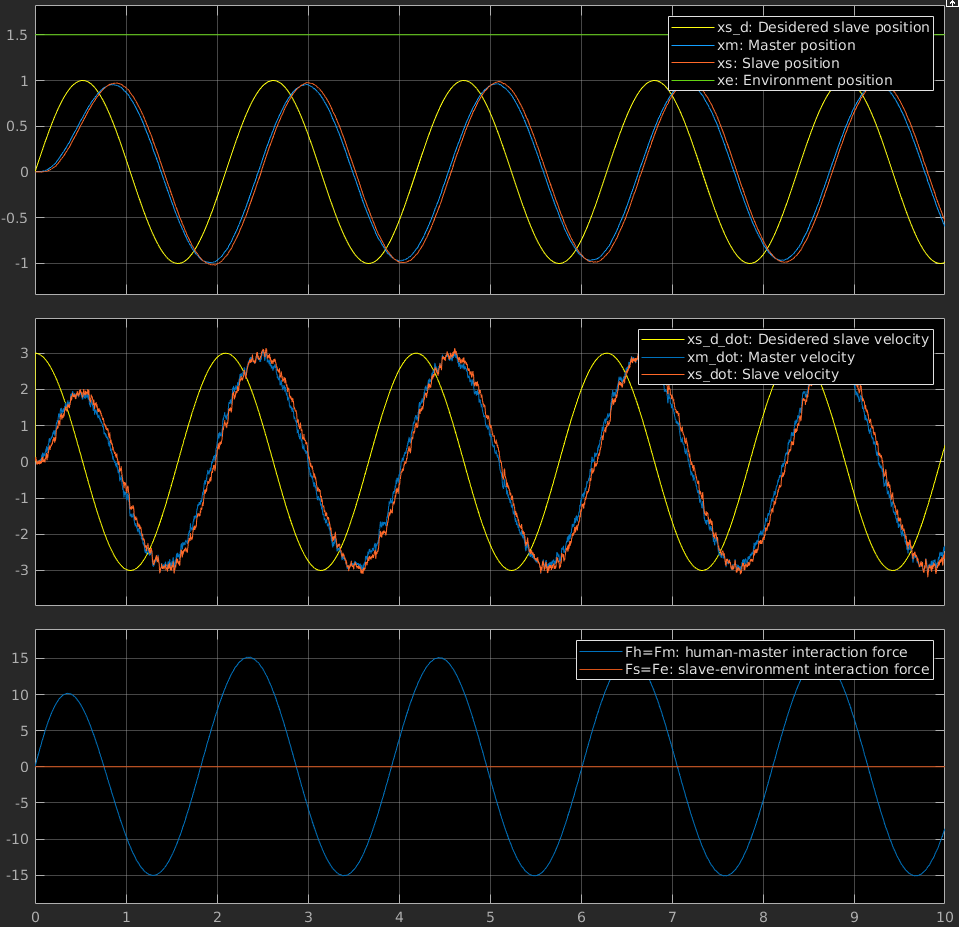
\includegraphics[keepaspectratio,width=\textwidth]{sfp_free_k}
\caption{FP in free motion, with noise}
\label{fig:sfp_free_k}

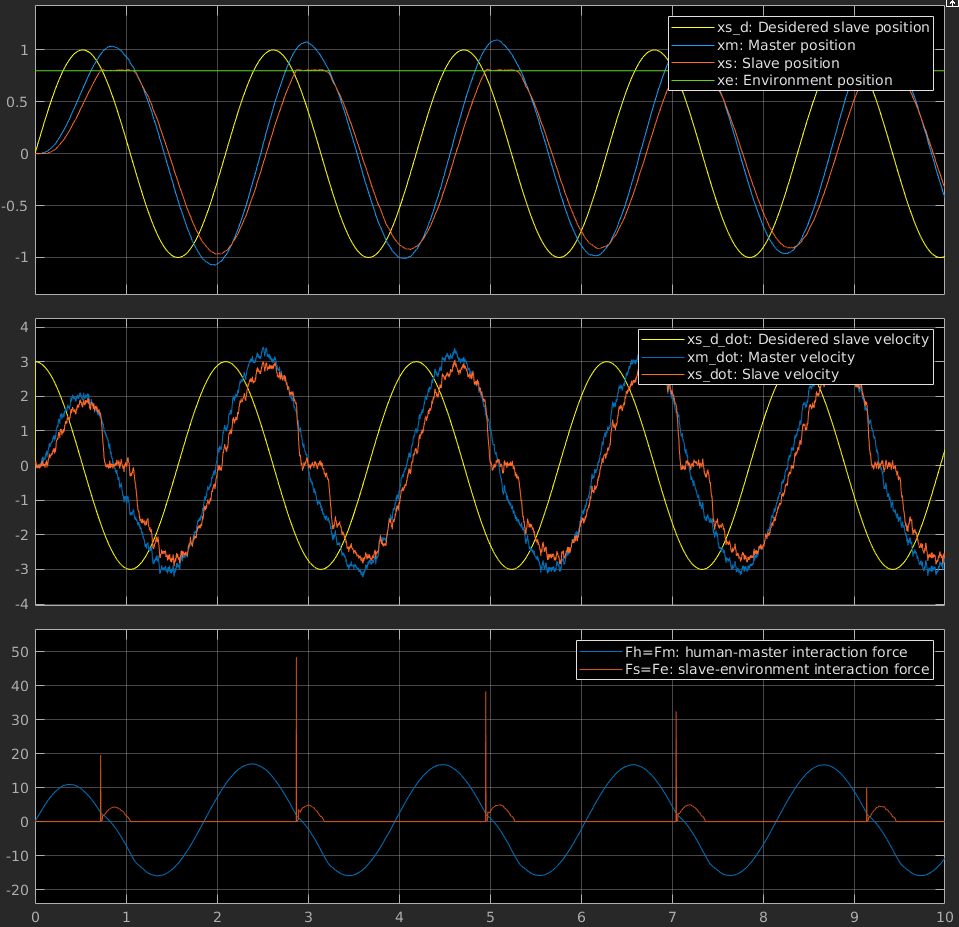
\includegraphics[keepaspectratio,width=\textwidth]{sfp_contact_k}
\caption{FP in contact, with noise}
\label{fig:sfp_contact_k}
\end{minipage}
\begin{minipage}{0.5\textwidth}
\centering
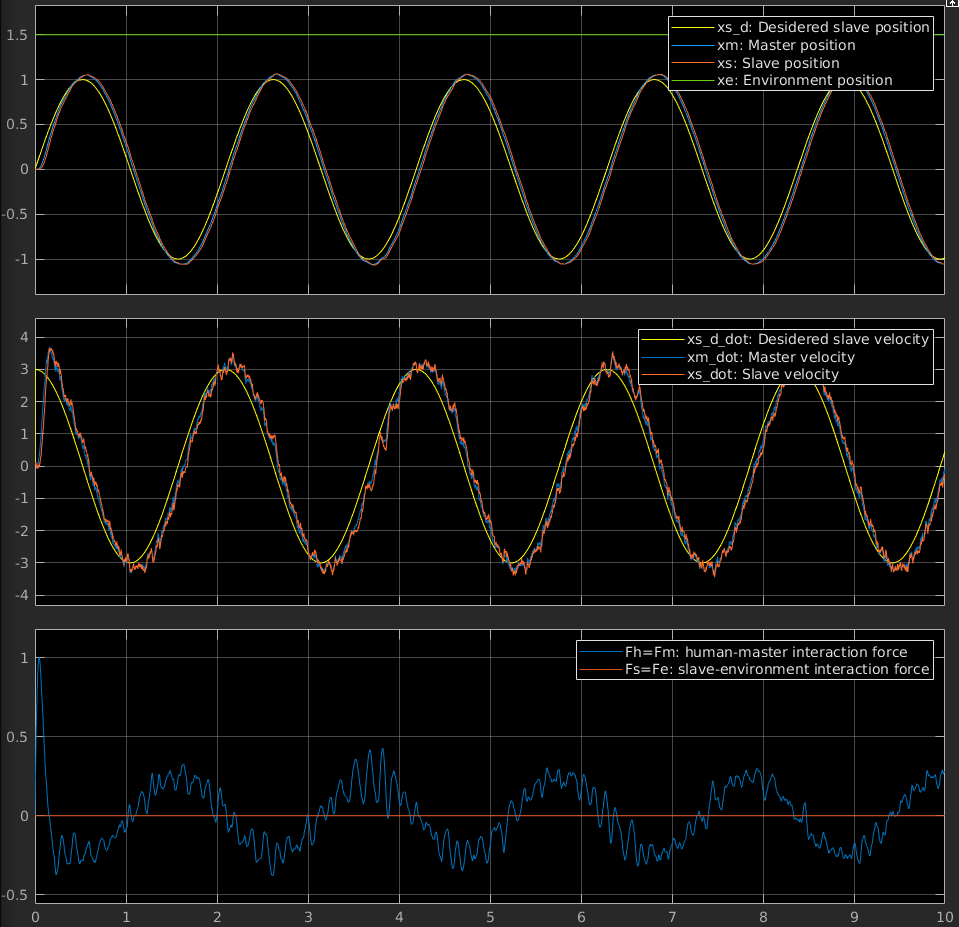
\includegraphics[keepaspectratio,width=\textwidth]{spp_free_k}
\caption{PP in free motion, with noise}
\label{fig:spp_free_k}

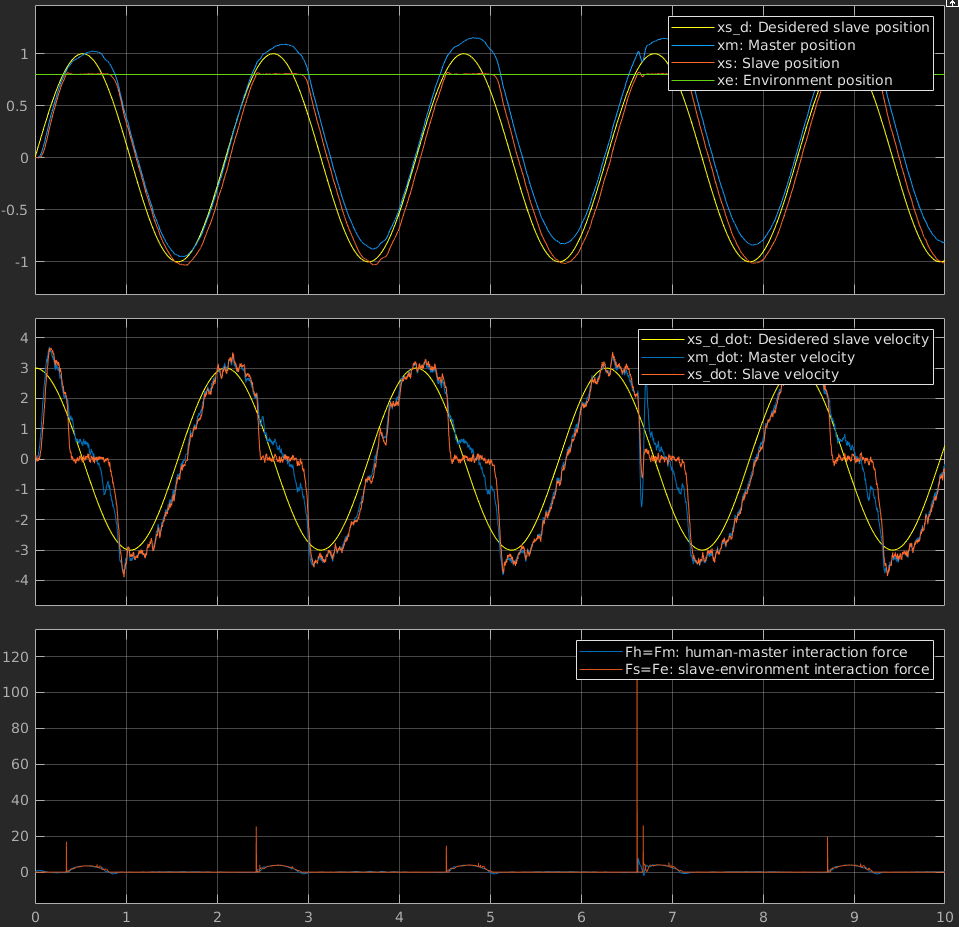
\includegraphics[keepaspectratio,width=\textwidth]{spp_contact_k}
\caption{PP in contact, with noise}
\label{fig:spp_contact_k}
\end{minipage}
\end{figure}

\newpage

\section{Assignment 7}

\subsection{Implement the Tank-based bilateral teleoperation architecture for the F-P and P-P cases}

\begin{figure}[h]
\centering
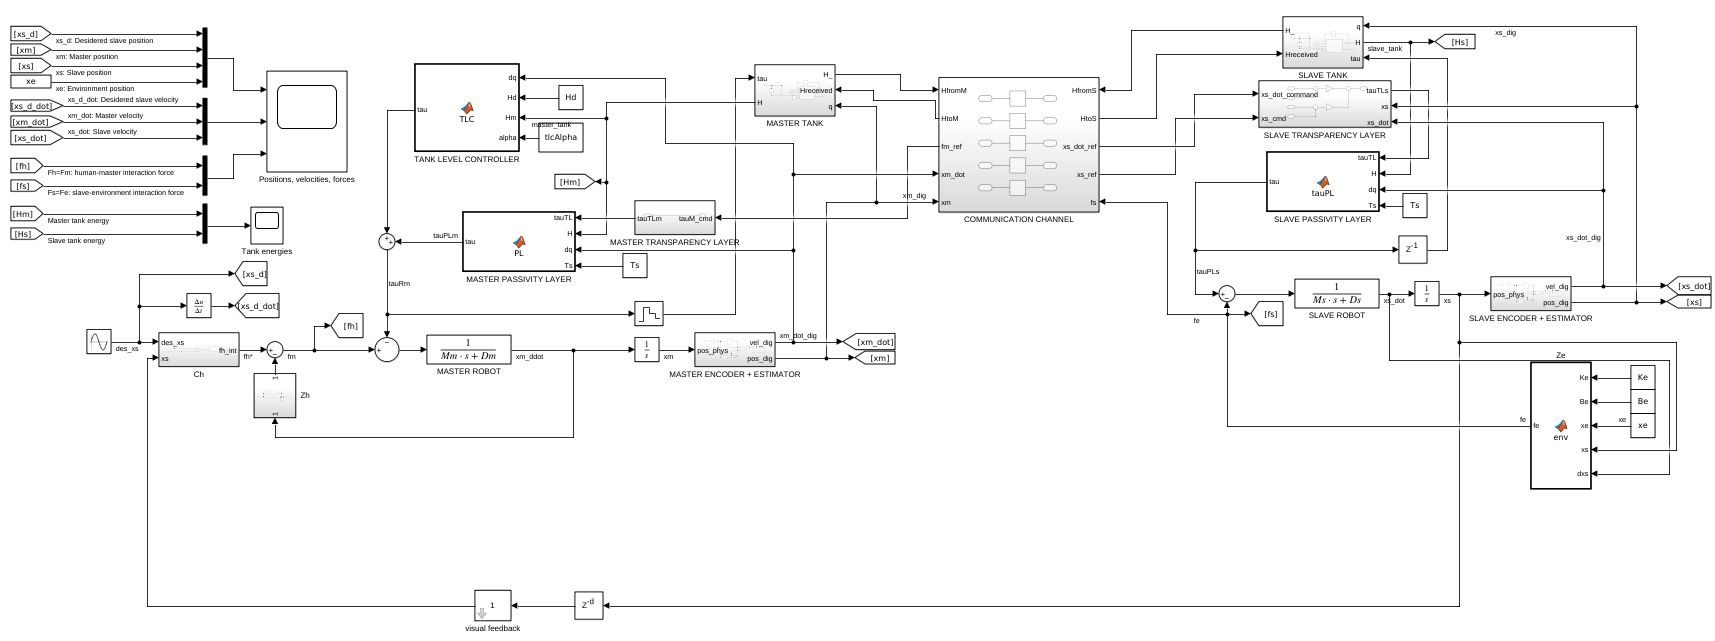
\includegraphics[keepaspectratio,width=\textwidth]{tank_fp}
\caption{Tank-based F-P teleoperation architecture}
\end{figure}

\begin{figure}[h]
\centering
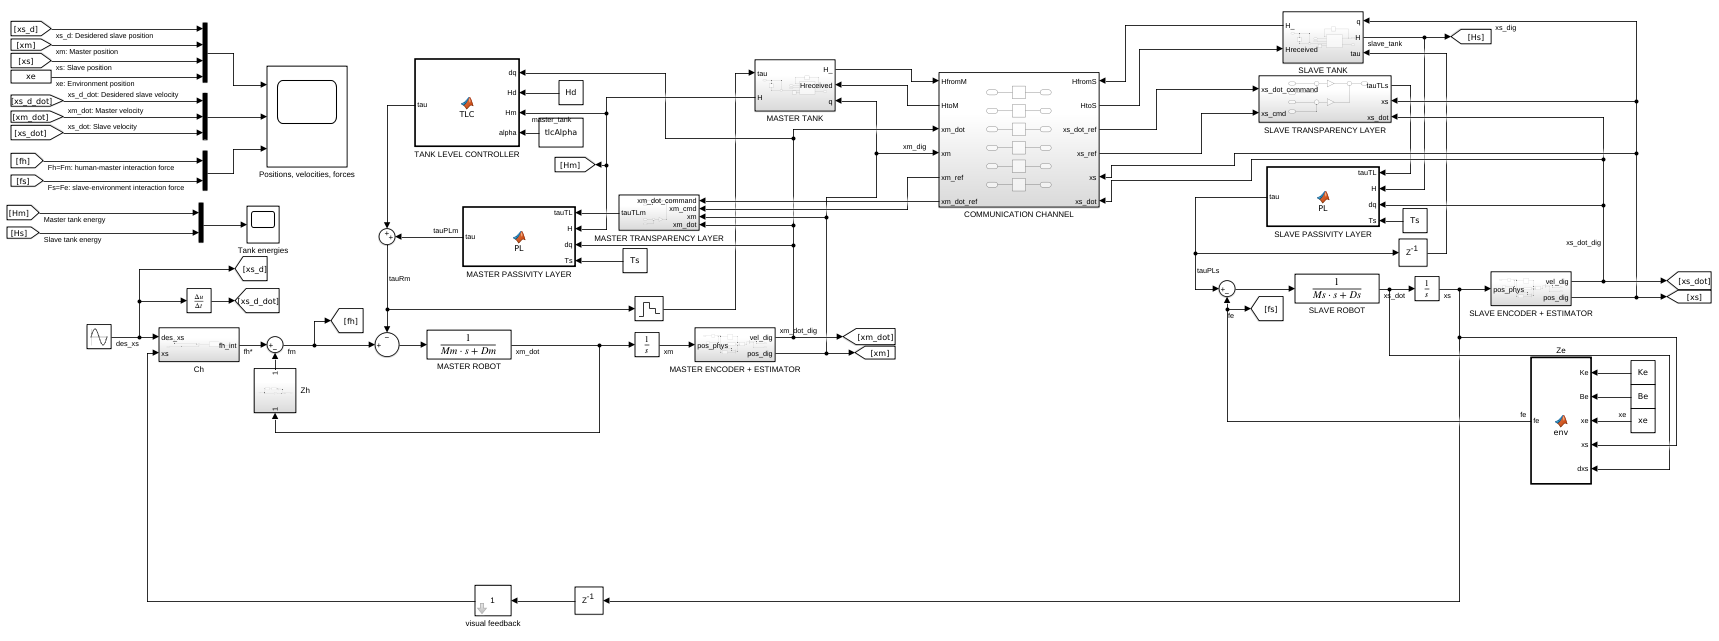
\includegraphics[keepaspectratio,width=\textwidth]{tank_pp}
\caption{Tank-based P-P teleoperation architecture}
\end{figure}

The tank-based teleoperation architecture uses a two-layer control architecture that combines passivity (and therefore stability) and transparency (and therefore high teleoperation performance). The layers, in hierarchical order, are:

\begin{itemize}
\item Passivity layer: introduces passivity, and therefore stability, into the system by absorbing the energy generated by communication delays or environment interaction forces.
\item Transparency layer: implements the control structure that ensures transparency of the teleoperation system, taking into account information about the system, environment and task the user is executing.
\end{itemize}

Both layers contribute some energy to an energy tank. The level of the tank represents the energy budget available to be used to carry out robot motions. The energy in the tank can only be replenished by the user at the master side.

To separate the passivity and transparency layers, a tank level controller (TLC) is introduced in the passivity layer at the master side. The role of the TLC is to regulate the tank's energy content,  ensuring it remains in a stable range. 

\subsection{Compare positions, velocities, forces, commands in free motion and in contact}

\begin{figure}[H]
\begin{minipage}{0.5\textwidth}
\centering
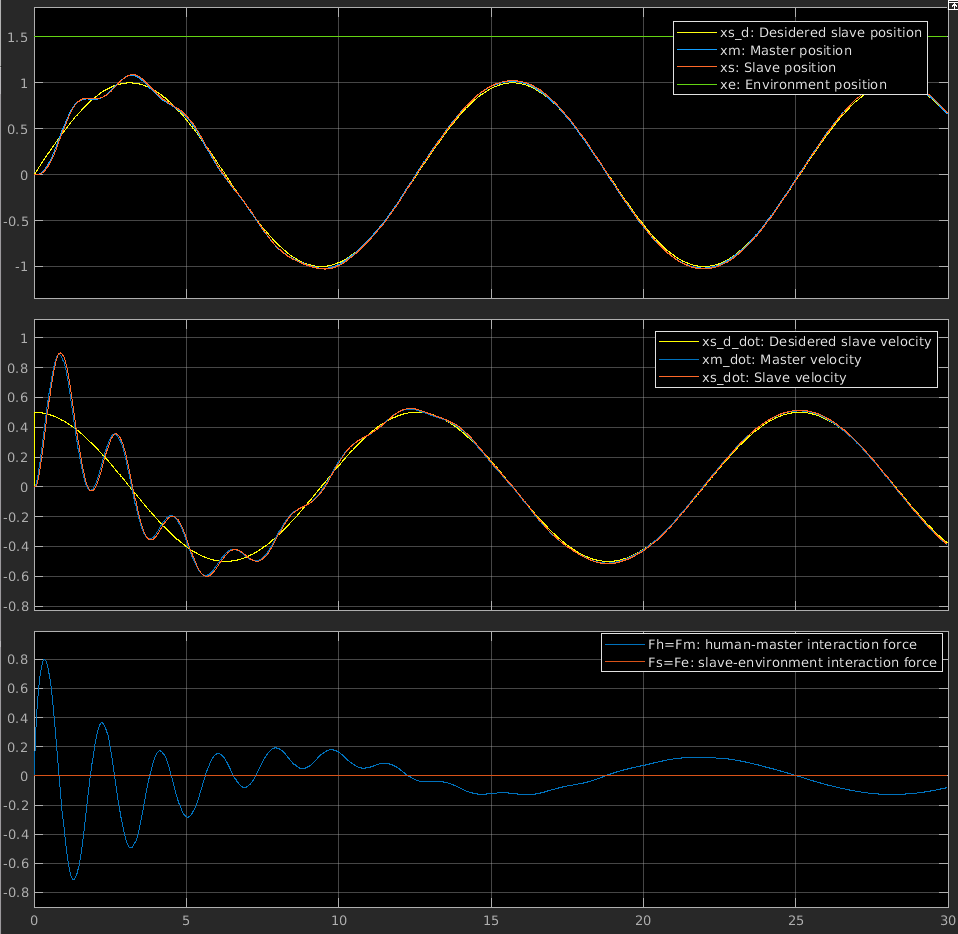
\includegraphics[keepaspectratio,width=\textwidth]{tfp_free_nok}
\caption{FP in free motion, without noise}
\label{fig:tfp_free_nok}

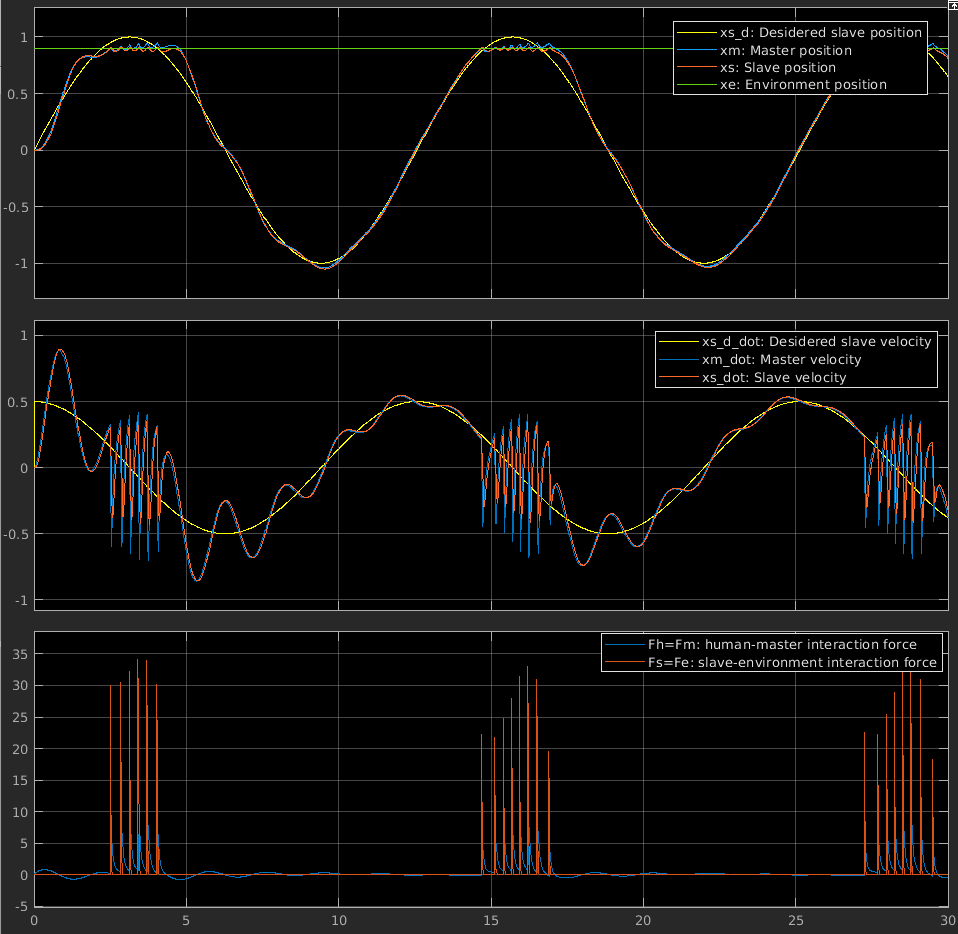
\includegraphics[keepaspectratio,width=\textwidth]{tfp_contact_nok}
\caption{FP in contact, without noise}
\label{fig:tfp_contact_k}
\end{minipage}
\begin{minipage}{0.5\textwidth}
\centering
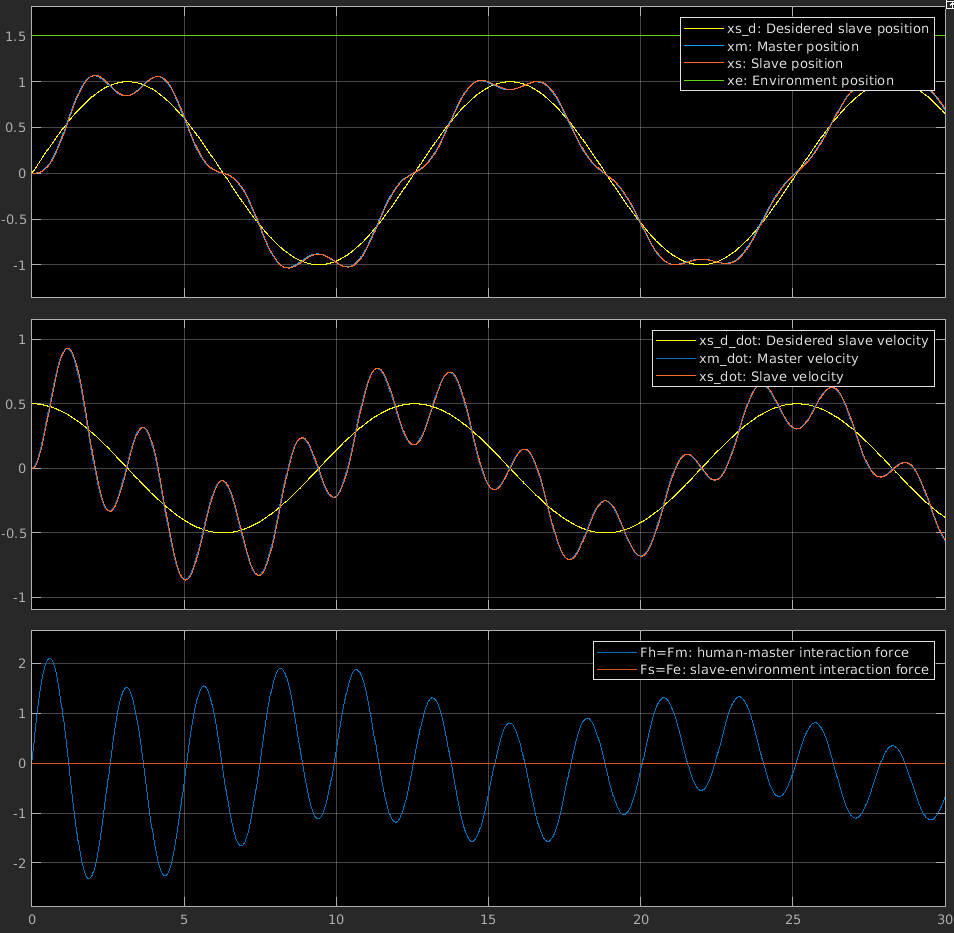
\includegraphics[keepaspectratio,width=\textwidth]{tpp_free_nok}
\caption{PP in free motion, without noise}
\label{fig:tpp_free_nok}

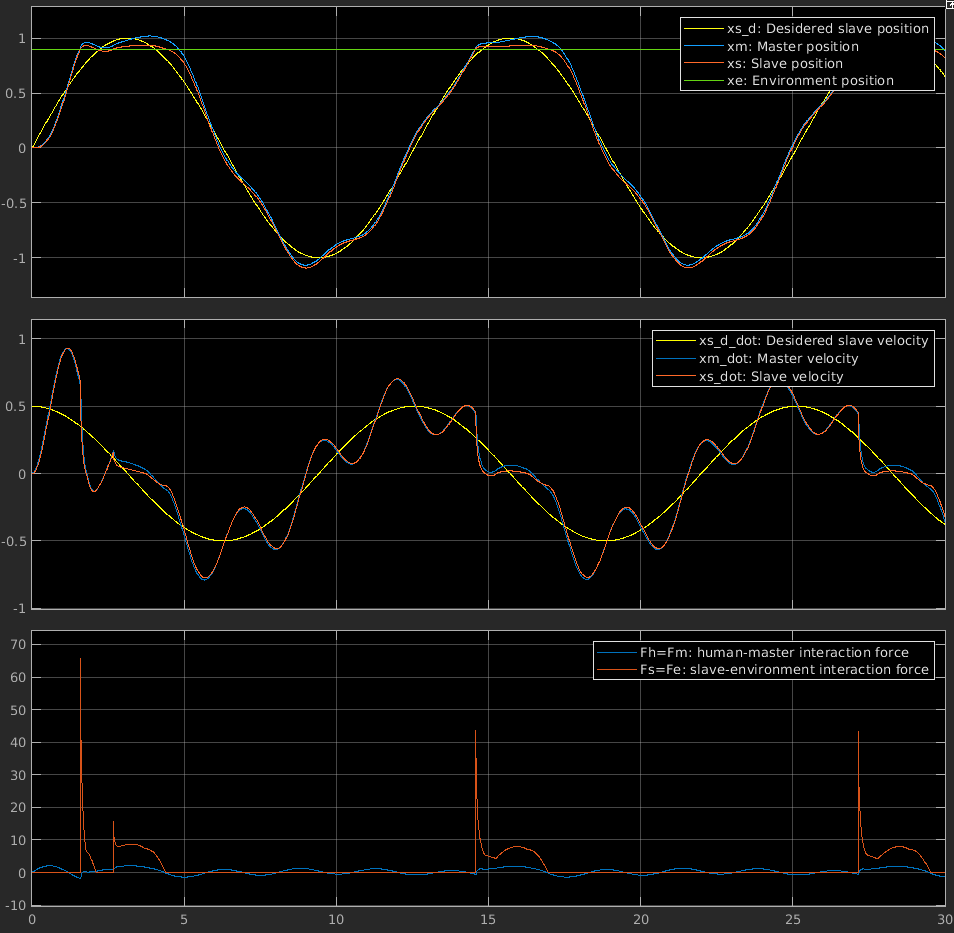
\includegraphics[keepaspectratio,width=\textwidth]{tpp_contact_nok}
\caption{PP in contact, without noise}
\label{fig:tpp_contact_nok}
\end{minipage}
\end{figure}

\subsection{Create another simulink model and (a) add the measurement noise to the position/force signals, and (b) estimate velocities from positions}

\begin{figure}[H]
\begin{minipage}{0.5\textwidth}
\centering
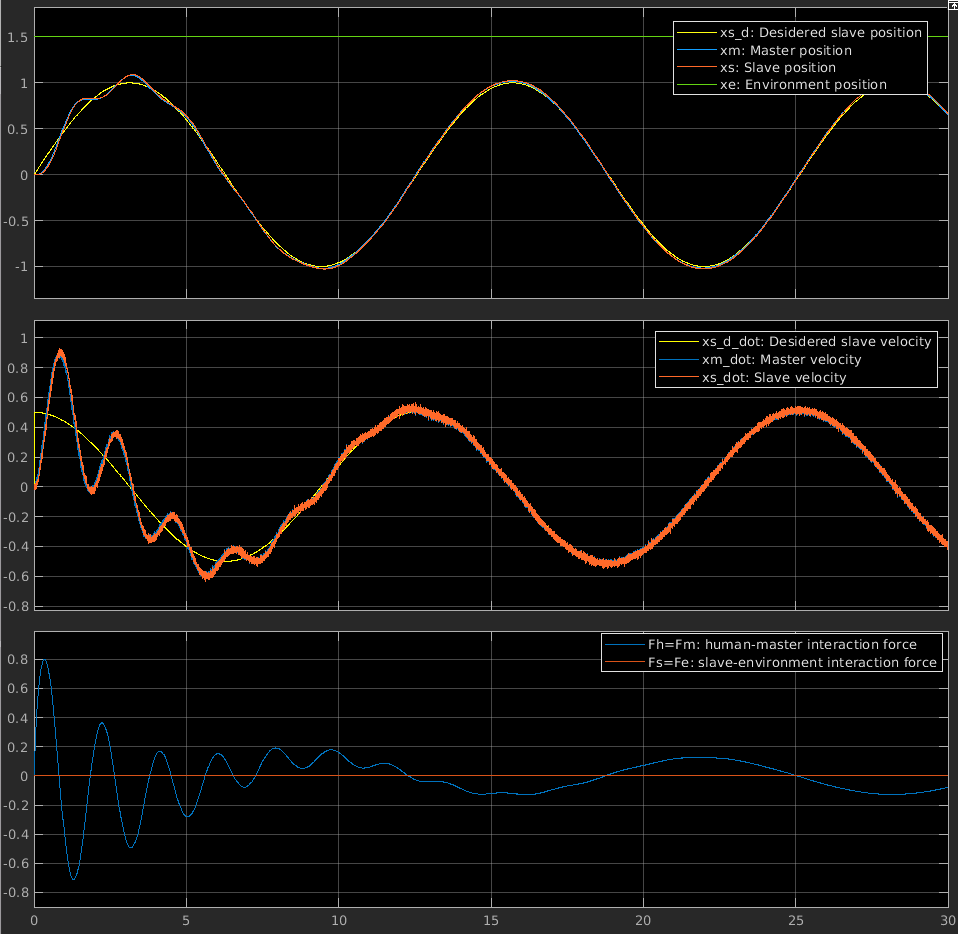
\includegraphics[keepaspectratio,width=\textwidth]{tfp_free_k}
\caption{FP in free motion, with noise}
\label{fig:spp_free_nok}

\includegraphics[keepaspectratio,width=\textwidth]{tfp_contact_k}
\caption{FP in contact, with noise}
\label{fig:spp_free_k}
\end{minipage}
\begin{minipage}{0.5\textwidth}
\centering
\includegraphics[keepaspectratio,width=\textwidth]{tpp_free_k}
\caption{PP in free motion, with noise}
\label{fig:spp_contact_nok}

\includegraphics[keepaspectratio,width=\textwidth]{tpp_contact_k}
\caption{PP in contact, with noise}
\label{fig:spp_contact_k}
\end{minipage}
\end{figure}

\subsection{PP - Tank energy levels}

\begin{figure}[H]
\begin{minipage}{0.5\textwidth}
\centering
\includegraphics[keepaspectratio,width=\textwidth]{tpp_free_energy}
\caption{Free motion, initial tank energy $H_m=H_s=15$}
\medskip
\includegraphics[keepaspectratio,width=\textwidth]{tpp_free_0energy}
\caption{Free motion, initial tank energy $H_m=H_s=0$}
\end{minipage}
\begin{minipage}{0.5\textwidth}
\centering
\includegraphics[keepaspectratio,width=\textwidth]{tpp_contact_energy}
\caption{Contact, initial tank energy $H_m=H_s=15$}
\medskip
\includegraphics[keepaspectratio,width=\textwidth]{tpp_contact_0energy}
\caption{Contact, initial tank energy $H_m=H_s=0$}
\end{minipage}
\end{figure}

\begin{figure}
\centering
\includegraphics[keepaspectratio,width=\textwidth]{tank_pp_longsim}
\caption{Free motion, initial tank energy $H_m=H_s=0$, longer simulation time}
\end{figure}

\begin{figure}
\centering
\includegraphics[keepaspectratio,width=\textwidth]{tank_pp_longsim_energy}
\caption{Free motion, initial tank energy $H_m=H_s=0$, longer simulation time}
\end{figure}

\newpage

\subsection{FP - Tank energy levels}

\begin{figure}[H]
\begin{minipage}{0.5\textwidth}
\centering
\includegraphics[keepaspectratio,width=\textwidth]{tfp_energy}
\caption{Free motion, initial tank energy $H_m=H_s=0.5$}
\end{minipage}
\begin{minipage}{0.5\textwidth}
\centering
\includegraphics[keepaspectratio,width=\textwidth]{tfp_energy_contact}
\caption{Contact, initial tank energy $H_m=H_s=0.5$}
\end{minipage}
\end{figure}


\end{document}